\chapter{Systematic Uncertainties}
\label{chap:Systematics}

Different sources of systematic uncertainty contribute to the estimation of background events and modeling of the signal. The chapter is organized as follows. Theoretical uncertainties concerning signals and major backgrounds are discussed in \autoref{sec:ThUnc}. Uncertainties concerning the \emph{nonprompt} background is discussed in \autoref{sec:NonUnc}. Uncertainties concerning the modeling of the diboson processes are discribed in \autoref{sec:DiUnc}. Finally, other systematic uncertainties are discussed in \autoref{sec:OthUnc}.
%%%%%%%%%%%%%%%%%%%%%%%%%%%%%%%%%%%%%%%%%%%%%%%%%%%%%%%%
%%%%%%%%%%%%%%%%%%%%%%%%%%%%%%%%%%%%%%%%%%%%%%%%%%%%%%%%

\section{Theoretical Uncertainties}
\label{sec:ThUnc}

Variations on theoretical cross sections for \emph{prompt} backgrounds are introduced to cover the uncertainties in perturbative \ac{QCD} calculations.  A 6$\%$ normalization uncertainty is assigned to WZ and ZZ processes~\cite{Campbell:2011bn}. A 15$\%$ normalization uncertainty is assigned to $\ttbar$W, $\ttbar$Z, and $\ttbar$H processes~\cite{Frederix:2021agh,Kulesza:2020nfh}. A 20$\%$ normalization uncertainty is assigned to tZq process, which is a conservative estimate taken from the MC generator. A conservative 50 $\%$ normalization uncertainty is assigned to other smaller \emph{prompt} backgrounds. All normalization uncertainties are considered uncorrelated between different processes but correlated between the years. 

Uncertainties associated to the \ac{PDF} are evaluated by using 100 replicas of the NNPDF sets~\cite{NNPDF:2014otw,NNPDF:2017mvq}. The procedure described in~\cite{CMS:2012nsv} is followed. Firstly, the sum of the generator weights of each replica is normalized to the nominal sum of the generator weights. This is done before any event selection to ensure no addtional normalization effect is introduced. After previous step, the bin-by-bin variations of the \ac{BDT} templates are obtained by calculating the bin-by-bin difference of the \ac{BDT} templates when switching from nominal \ac{PDF} to each \ac{PDF} replica. Finally, \ac{PDF} uncertainty for each bin is assigned by taking the root mean square value of the 100 variations of the corresponding bin. This uncertainty is treated as uncorrelated between different processes but correlated between the years.  We consider this uncertainty for all the signals and major prompt backgrounds (i.e. WZ, $\ttbar$W, $\ttbar$Z, and $\ttbar$H).

\ac{QCD} scale uncertainties are evaluated by varying the renormalization scale $\mu_\textsf{R}$ and factorization scales $\mu_\textsf{F}$ in \ac{ME}.  A total of six variations are considered: varying $\mu_\textsf{R}$ by a factor of 2 and 0.5, varying $\mu_\textsf{F}$ by a factor of 2 and 0.5, and varying $\mu_\textsf{R}$ and $\mu_\textsf{F}$ simultaneously by a factor of 2 and 0.5. Similar to PDF uncertainty, normalization effects of each variation is removed. An envelope that covers all six variations is used to represent the scale uncertainty. This uncertainty is treated as uncorrelated between different processes but correlated between the years. We consider this uncertainty for all the signals and major prompt backgrounds (i.e. WZ, $\ttbar$W, $\ttbar$Z, and $\ttbar$H).

Uncertainties associated to the \ac{PS} are evaluated by varying the renormalization scale $\mu_\textsf{R}$ in the initial and final state radiations, which effectively changes the strong coupling constant in the \ac{PS}. Similarly, $\mu_\textsf{R}$ is varied by a factor of 2 and 0.5, and normalization effects of each variation is removed. This uncertainty is treated as uncorrelated between different processes but correlated between the years.  We consider this uncertainty for all the signals and major prompt backgrounds (i.e. WZ, $\ttbar$W, $\ttbar$Z, and $\ttbar$H).
%%%%%%%%%%%%%%%%%%%%%%%%%%%%%%%%%%%%%%%%%%%%%%%%%%%%%%%%
%%%%%%%%%%%%%%%%%%%%%%%%%%%%%%%%%%%%%%%%%%%%%%%%%%%%%%%%

\section{Nonprompt Uncertainties}
\label{sec:NonUnc}

There are several sources of uncertainties associated to the determination of the \emph{nonprompt} efficiency $f$. One of these uncertainties comes from the estimate of \emph{prompt} contamination in \ac{MR}. As is discussed in \autoref{chap:Nonprompt}, \emph{prompt} backgrounds (estimated with \ac{MC}) are subtracted from total event yields measured in data. A flat 20 $\%$ uncertainty ($\alpha$ in Equation \ref{eq:f_eq}) is assigned to the event yields of the \emph{prompt} background and the resulting variation of $f$ is taken as the uncertainty.

\begin{equation}
f=\frac{n_{data}^{tag+tight}-(1+\alpha)n_{MC(prompt)}^{tag+tight}}{n_{data}^{tag+loose}-(1+\alpha)n_{MC(prompt)}^{tag+loose}}.
\label{eq:f_eq}
\end{equation}  

\begin{figure}[tbh!]
 \begin{center}
 \begin{tabular}{c}
 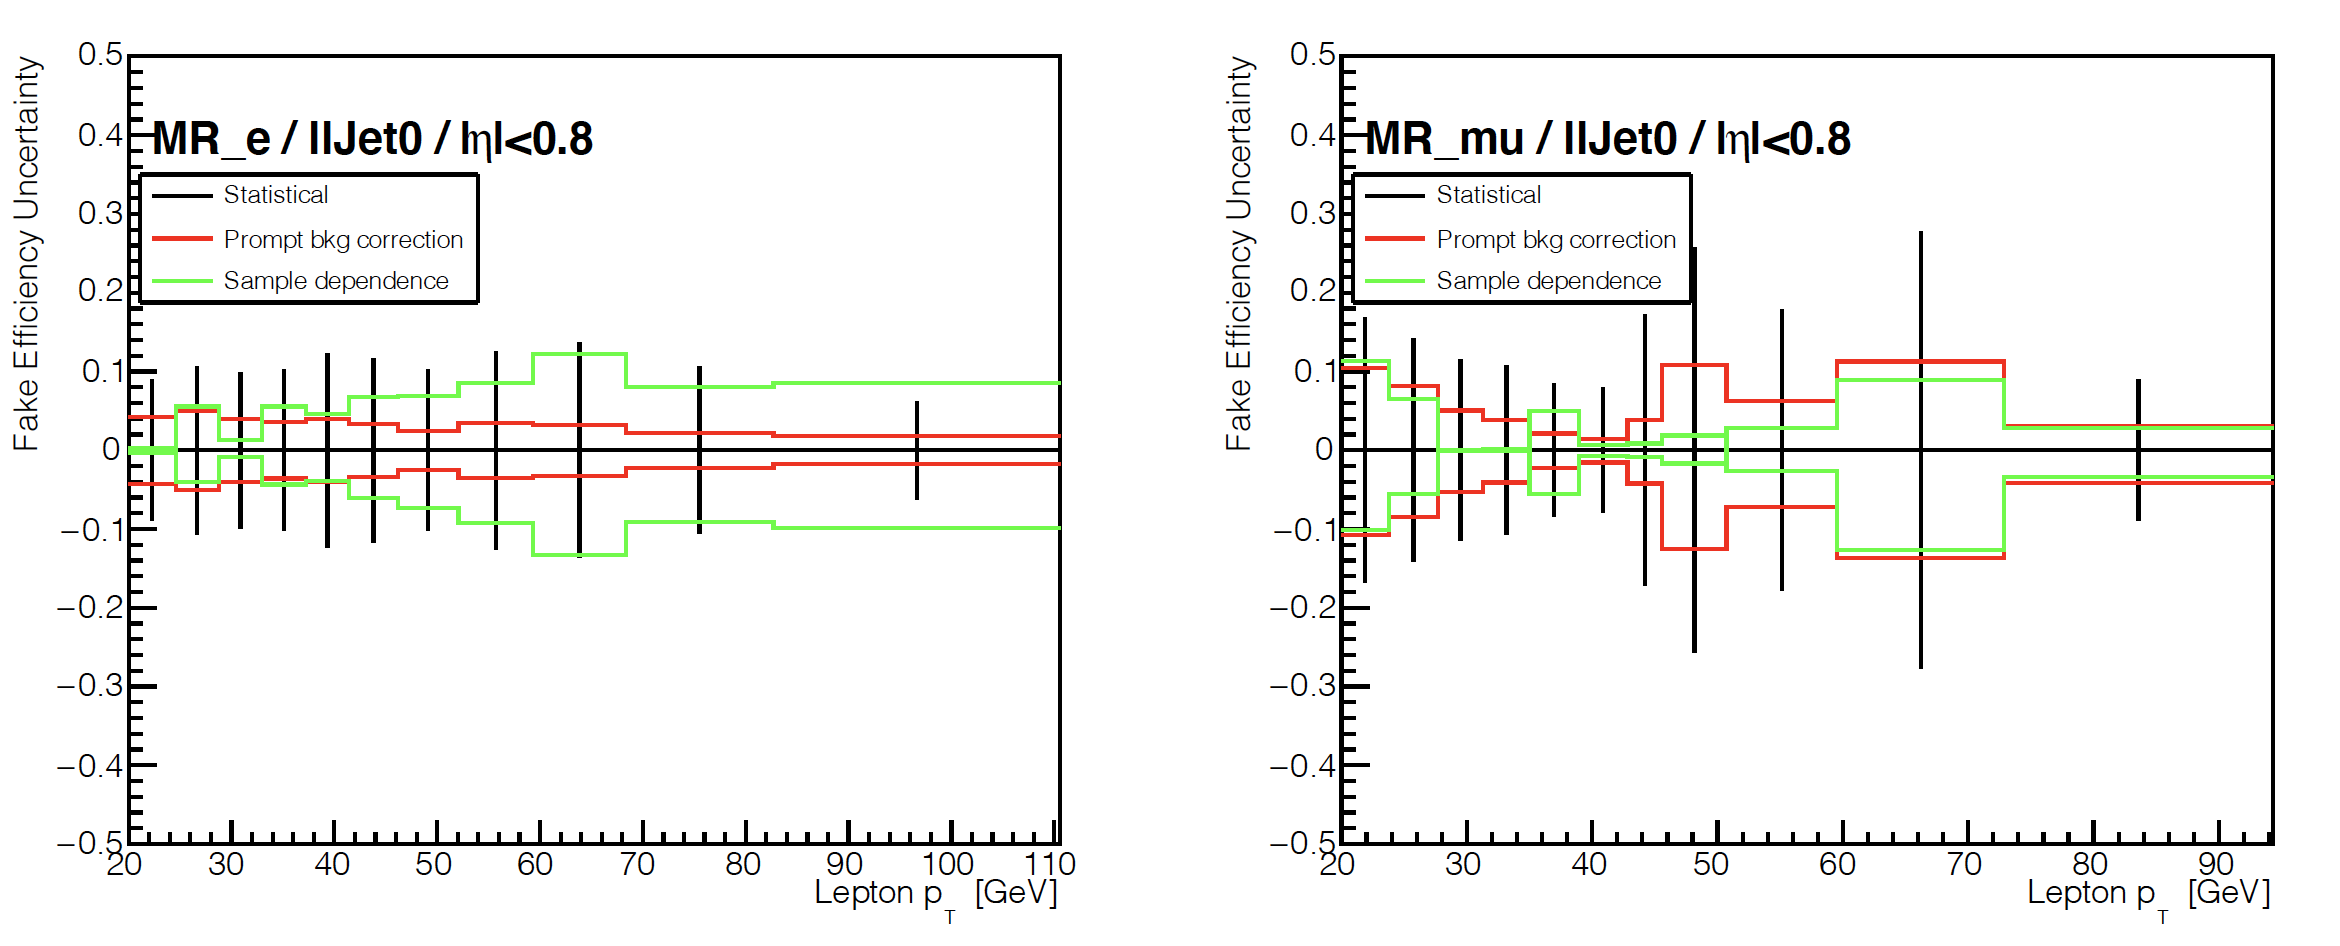
\includegraphics[width=0.99\textwidth]{figures/Part3/Systematics/MR1}
 \end{tabular}
 \caption{Comparison of different components of the uncertainties associated to the \emph{nonprompt} efficiency measured in 2017 dataset (njet=0 bin, $|\eta|<$0.8 bin). From left to right: electron $f$ uncertainty, muon $f$ uncertainty.}
 \label{fig:f_comp1}
 \end{center}
\end{figure}

Another source of uncertainty associated to the determination of \emph{nonprompt} efficiency \emph{f} is concerned with the observation that f exhibits a flavor-dependency, as is shown in Figure~\ref{fig:fake_eff}. This can happen when different physics processes enter \acp{MR} with different lepton flavor composites, which lead to differences in \emph{nonprompt} lepton behaviors. This type of uncertainty, referred to as ``sample dependence'', is estimated by introducing a variation factor $\beta$ between the proportions of same-flavor and different-flavor pairs in \ac{MR}. For example, electron \emph{f} can be calculated as (prompt background correction is ignored from the equation),

\begin{equation}
f_{\textsf{e}}=\frac{(1+\beta)n_{\textsf{e+e}}^{tag+tight}+(1-\beta)n_{\textsf{e+}\upmu}^{tag+tight}}{(1+\beta)n_{\textsf{e+e}}^{tag+loose}+(1-\beta)n_{\textsf{e+}\upmu}^{tag+loose}}.
 \label{eq:samp_dep}
\end{equation}

A 20$\%$ variation ($\beta$) is assigned the resulting variation of $f$ is taken as the uncertainty.
 
Statistical uncertainty is also considered when determining $f$. A comparison of different sources of uncertainties are shown in Figure \ref{fig:f_comp1} and Figure \ref{fig:f_comp2}. All sources of uncertainties are added in quadrature to form the final uncertainty on $f$. 

\begin{figure}[tbh!]
 \begin{center}
 \begin{tabular}{c}
 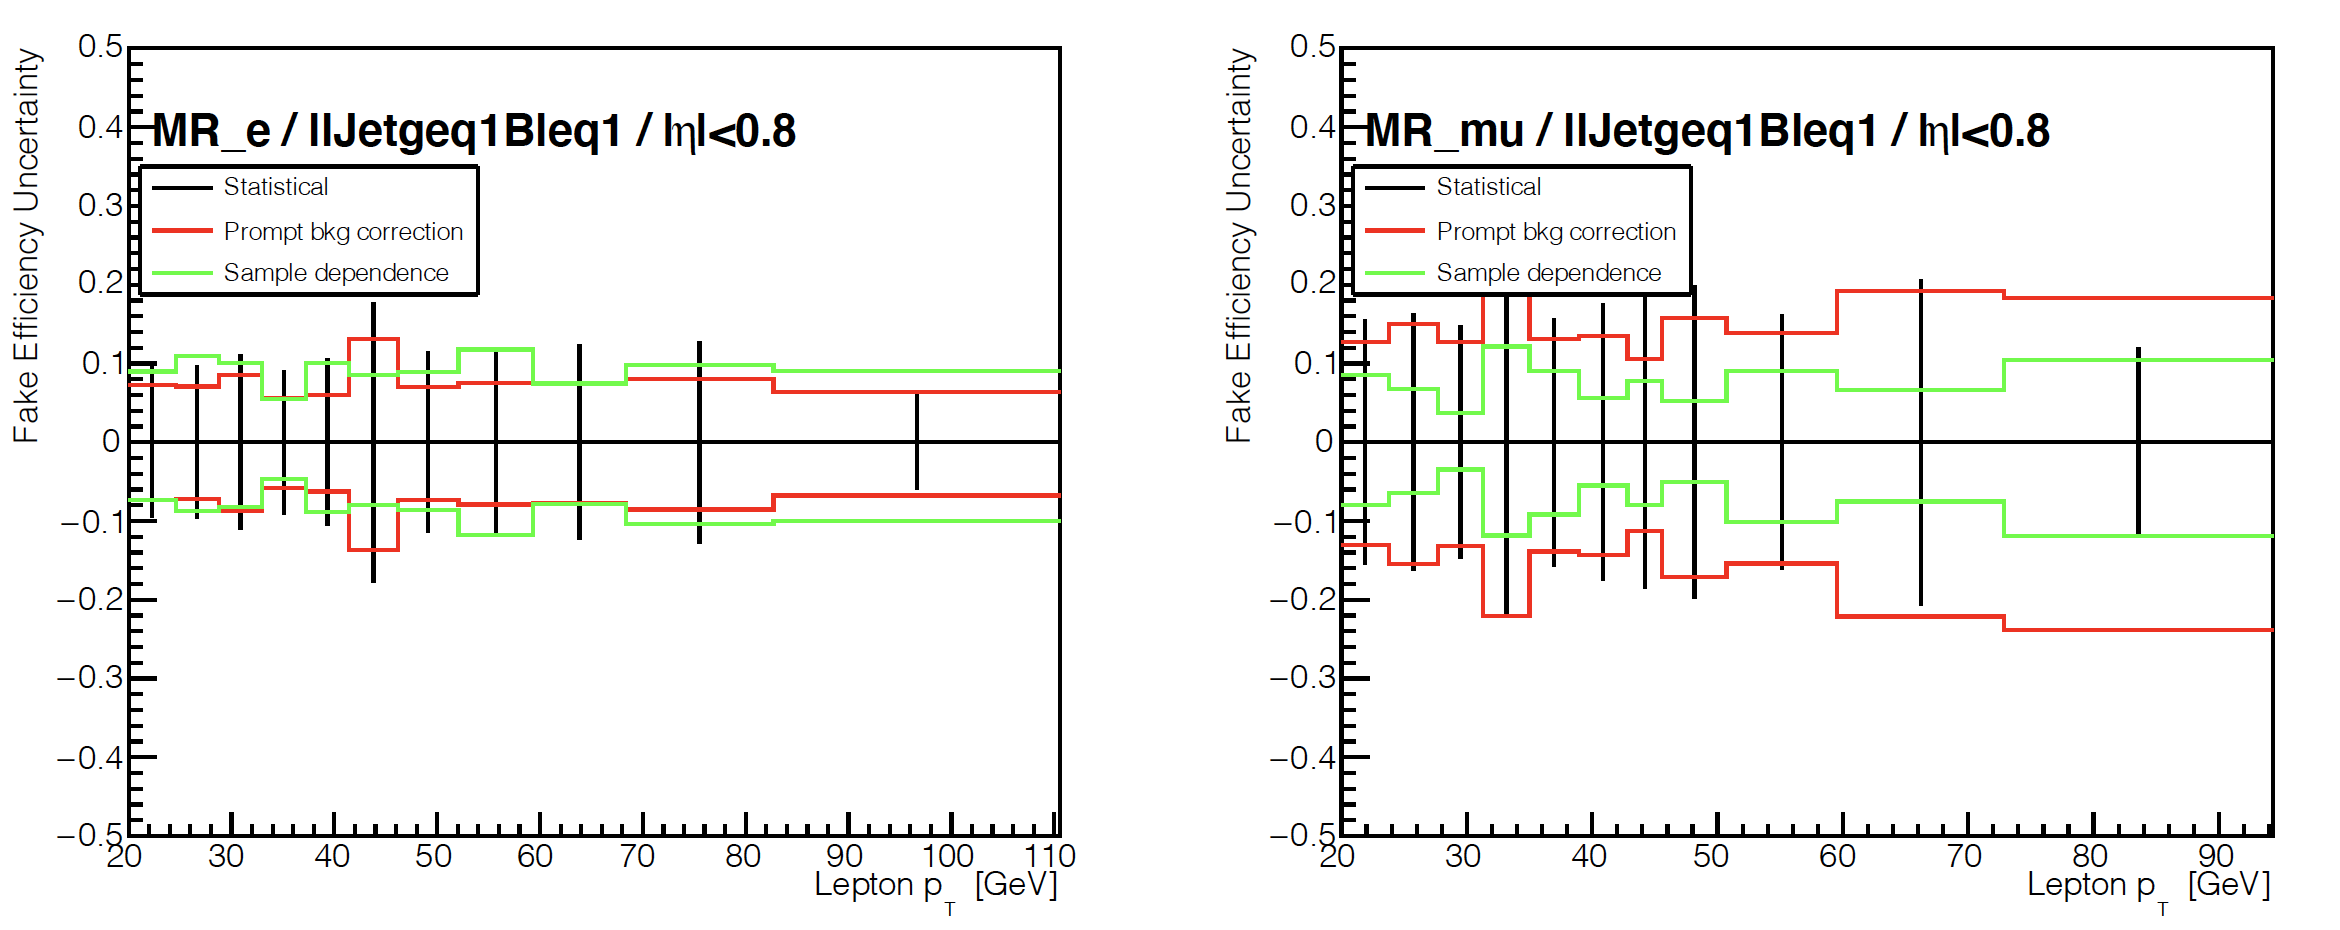
\includegraphics[width=0.99\textwidth]{figures/Part3/Systematics/MR2}
 \end{tabular}
 \caption{Comparison of different components of the uncertainties associated to the \emph{nonprompt} efficiency measured in 2017 dataset (njet$>$0 bin, $|\eta|<$0.8 bin). From left to right: electron $f$ uncertainty, muon $f$ uncertainty.}
 \label{fig:f_comp2}
 \end{center}
\end{figure}

Since the \emph{prompt} efficiency $r$ is measured in simulated $\ttbar$ events, \ac{MC} uncertainties described in \autoref{sec:OthUnc} are propagated to $r$ as the uncertainties. Additionally, statistical uncertainty is added in quadrature to the MC uncertainties to form the final uncertainty on $r$.

The uncertainties associated to the \emph{prompt} efficiency are relatively small when compared to the \emph{nonprompt} efficiency uncertainties. A comparison of different sources of \emph{prompt} efficiency uncertainties are shown in Figure \ref{fig:r_comp}.

\begin{figure}[tbh!]
 \begin{center}
 \begin{tabular}{c}
 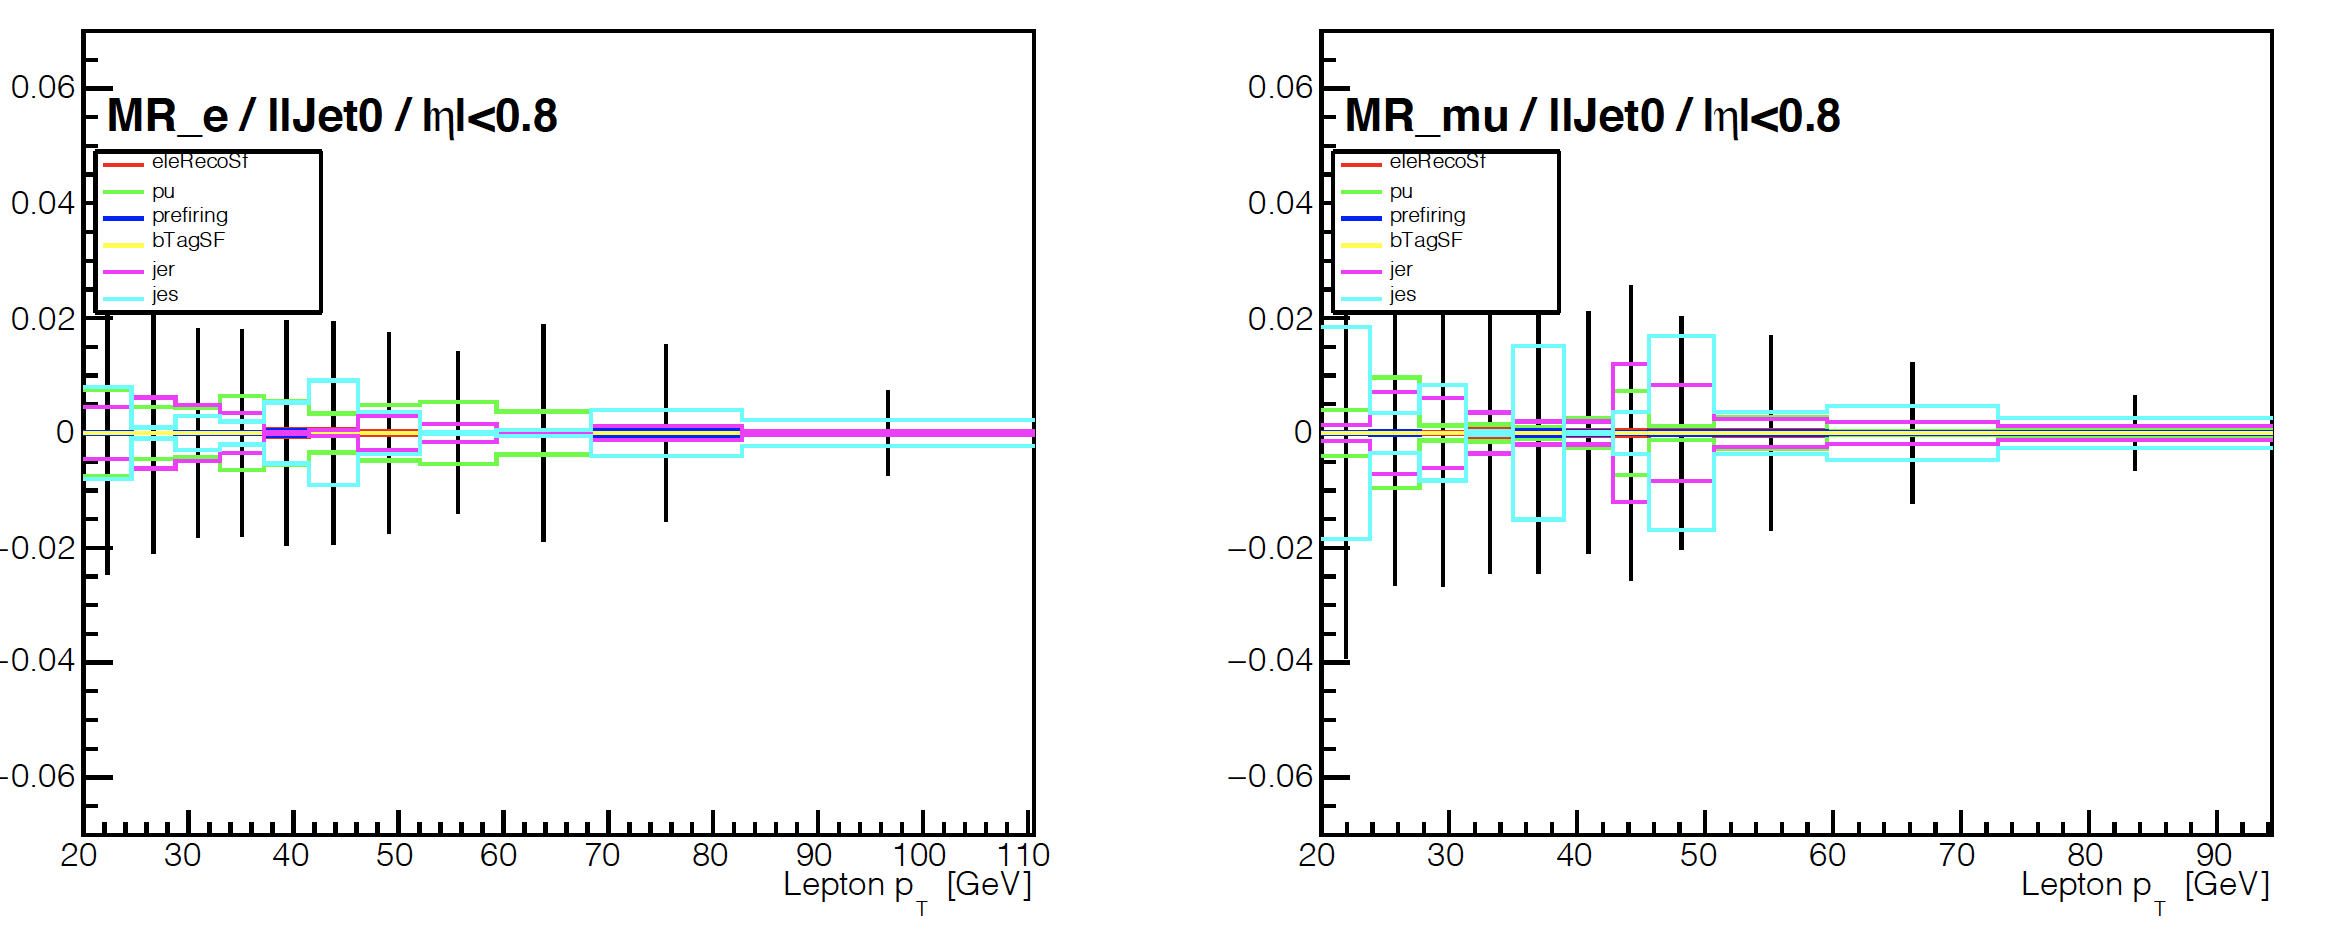
\includegraphics[width=0.99\textwidth]{figures/Part3/Systematics/MR}
 \end{tabular}
 \caption{Comparison of different components of the uncertainties associated to the \emph{prompt} efficiency measured in 2017 dataset (njet$=$0 bin, $|\eta|<$0.8 bin). From left to right: electron $r$ uncertainty, muon $r$ uncertainty.}
 \label{fig:r_comp}
 \end{center}
\end{figure}

Uncertainties associated to $r$ and $f$ are determined separately for electron and muon. Therefore, there are four independent uncertainties: $r_{\textsf{e}}$, $r_{\upmu}$, $f_{\textsf{e}}$ and $f_{\upmu}$. 

A fifth uncertainty is considered that accounts for the potential bias caused by the way the generalized matrix method is implemented. Four out of the eight \acp{AR} that appear on the lefthand side of the Equation \ref{eq:matrix_method3} (i.e. $N^{\overline{T}TT}$, $N^{\overline{T}T\overline{T}}$, $N^{\overline{T}\overline{T}T}$, $N^{\overline{T}\overline{T}\overline{T}}$) are selected by requiring the leading lepton in $\pt$ to fail the \emph{tight} criteria described in Table~\ref{tab:looseandtight}. Effectively this means that the isolation requirement is reversed for leading lepton that enter these four \acp{AR}. Selecting the leading lepton by a loose requirement is not ideal since the leading lepton is required to match with iso-triggers. To account for this bias, a 50 $\%$ uncertainty is assigned to the $f_1$ (\emph{nonprompt} efficiency associated to the leading lepton) for events that enter these four \acp{AR}. The variation of the \emph{nonprompt} estimate due to trigger matching is largely covered by this uncertainty, as is shown in Figure~\ref{fig:MM_trigger}.

\begin{figure}[tbh!]
 \begin{center}
 \begin{tabular}{cc}
 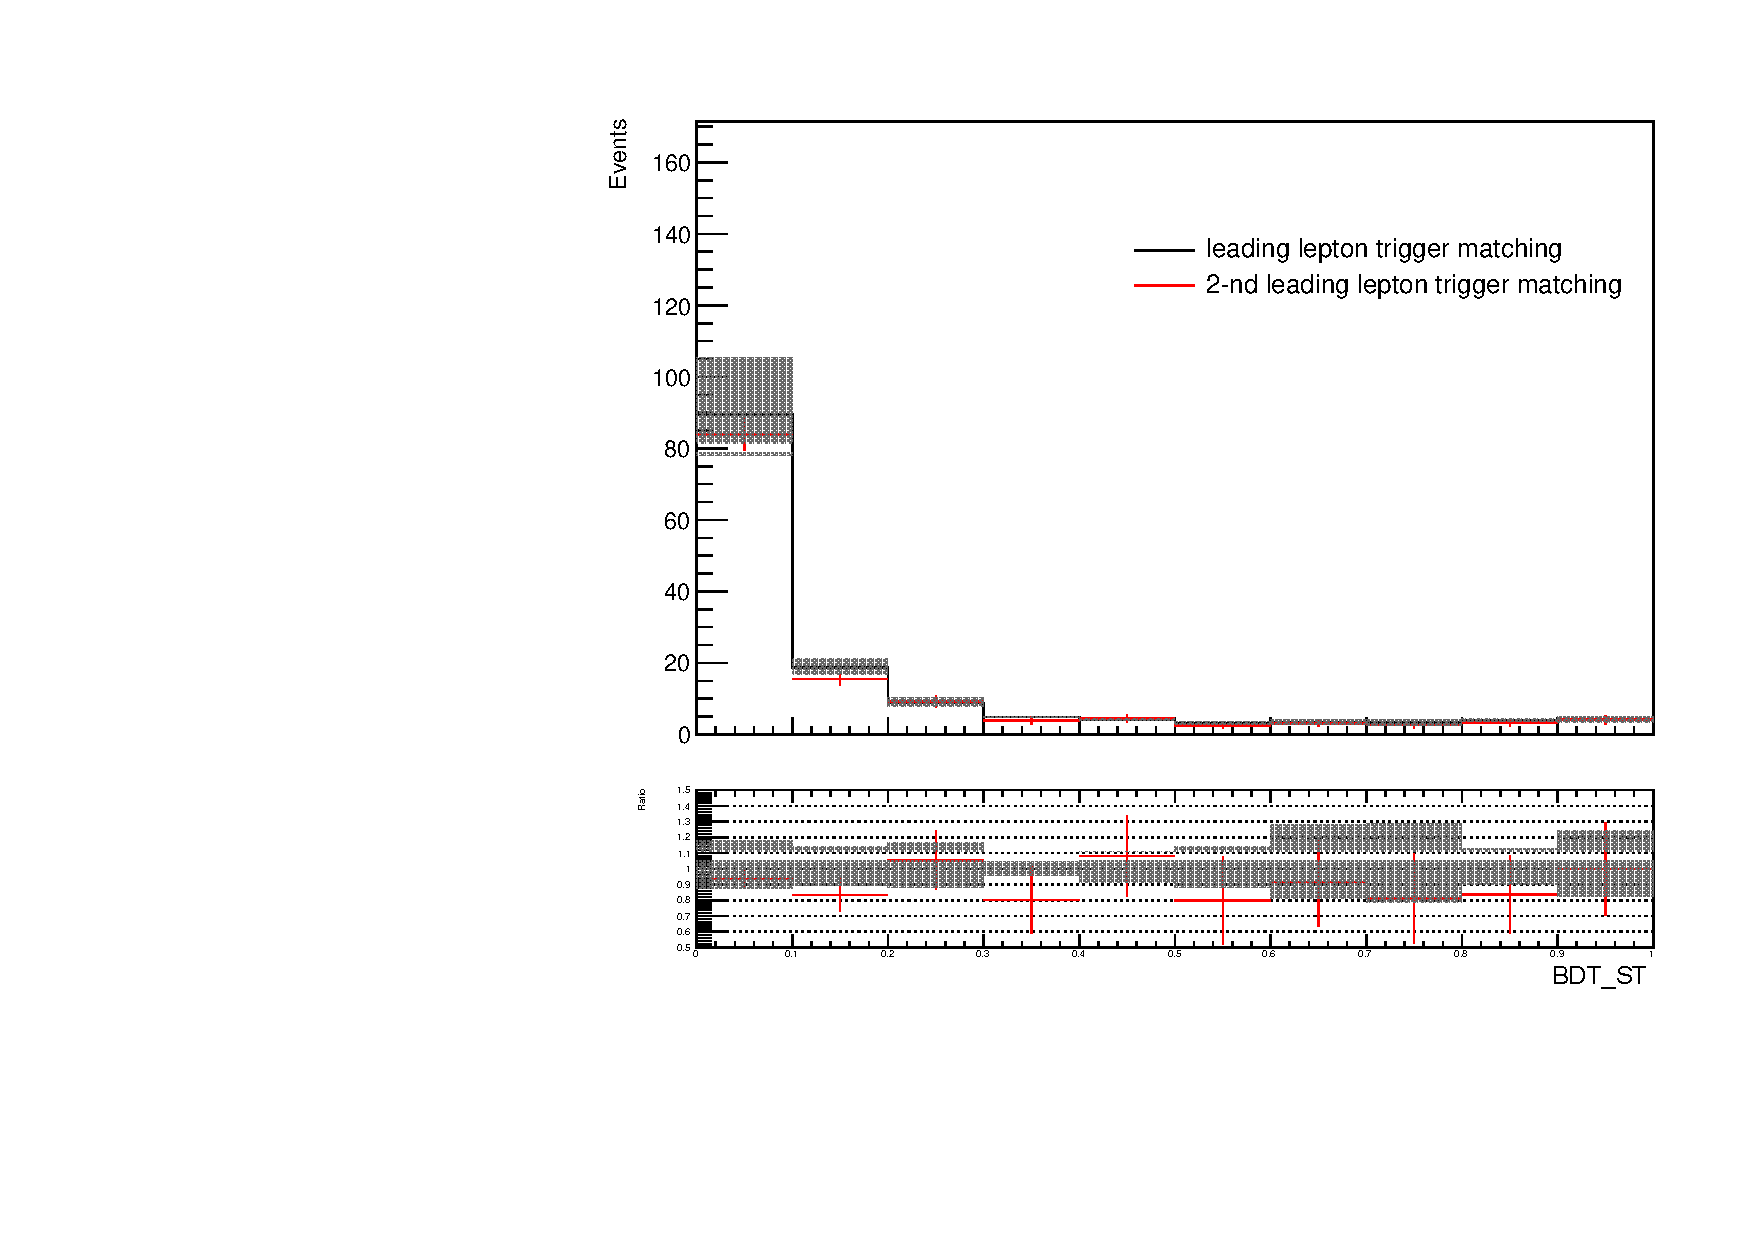
\includegraphics[width=0.47\textwidth]{figures/Part3/Systematics/BDT_ST_MM}&
 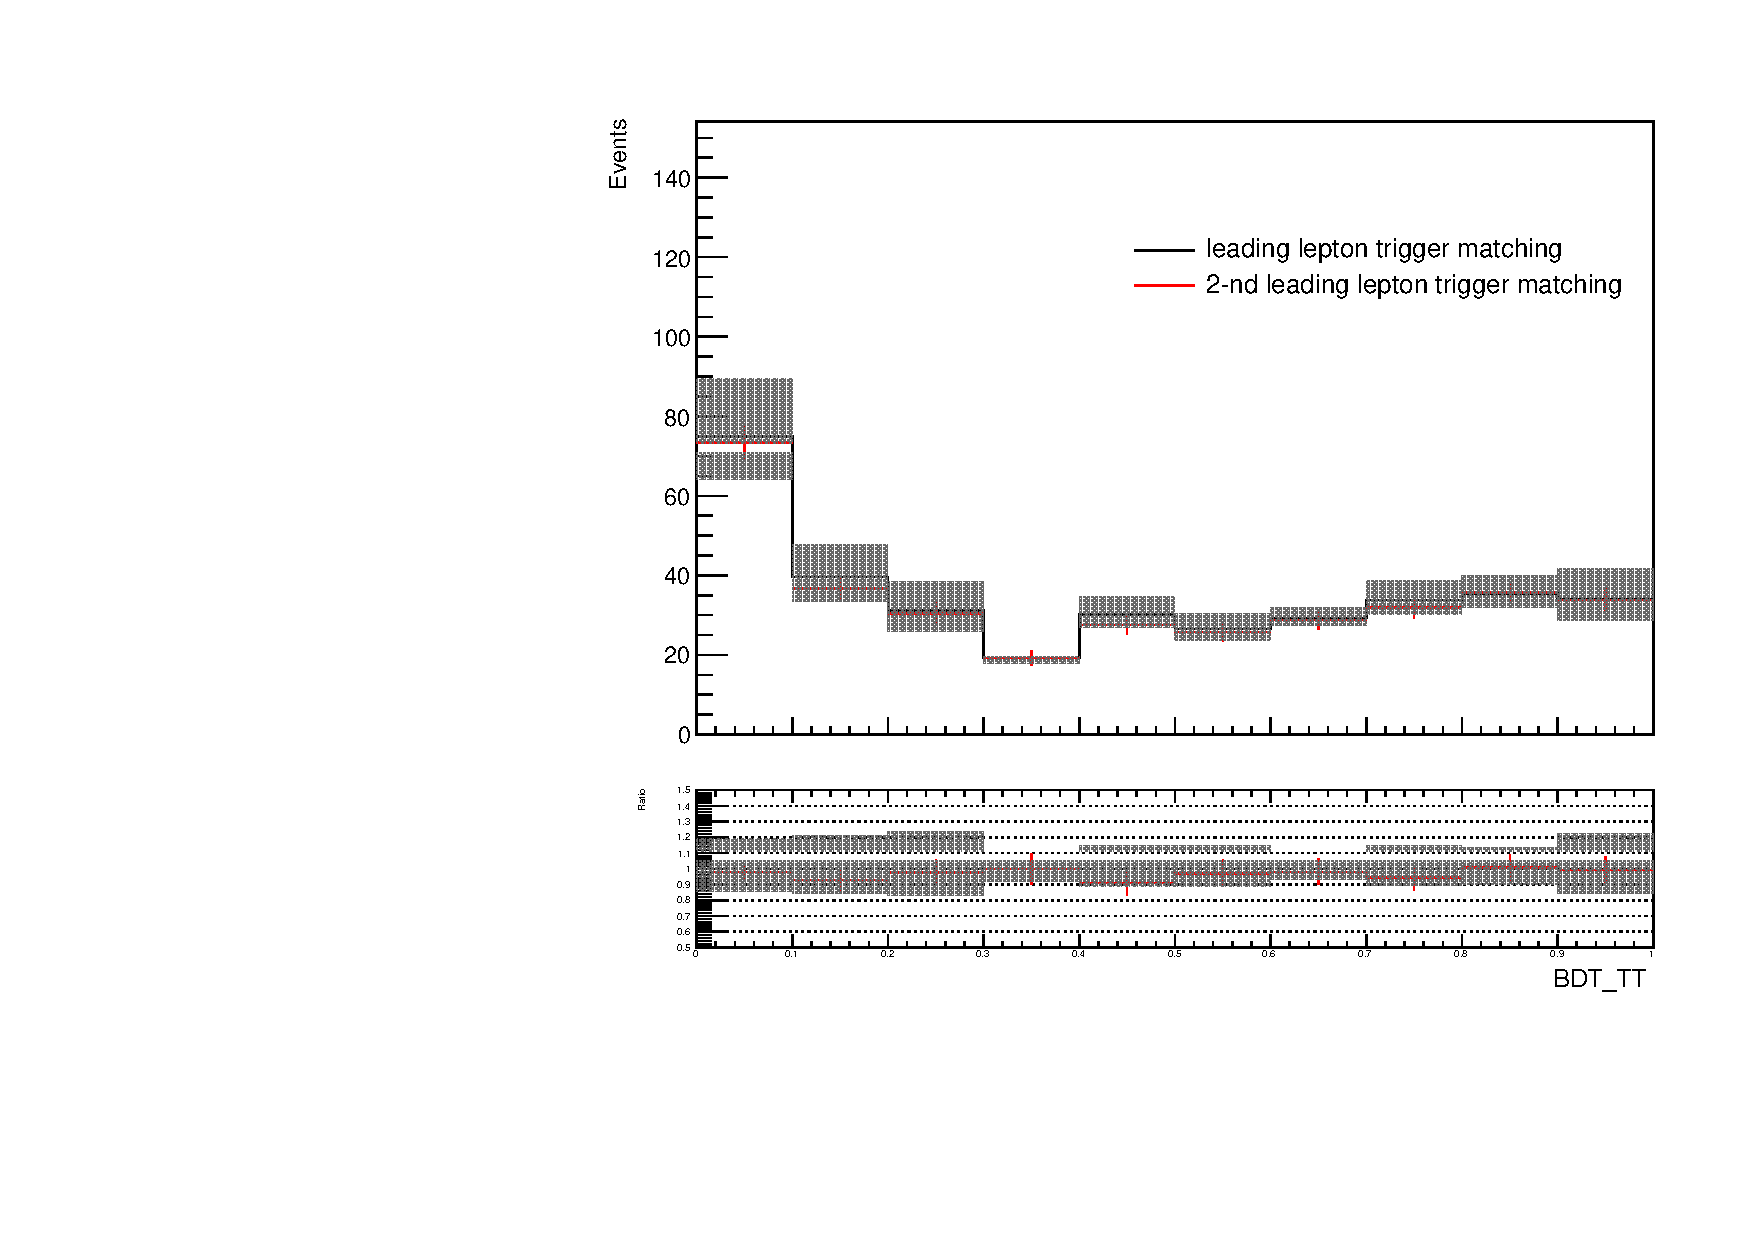
\includegraphics[width=0.47\textwidth]{figures/Part3/Systematics/BDT_TT_MM} \\
 \end{tabular}
 \caption{The impact of matching leptons to trigger objects on \emph{nonprompt} estimate. From left to right: \emph{nonprompt} estimate in top production enriched \ac{SR}, \emph{nonprompt} estimate in top decay enriched \ac{SR}. The nominal configuration of the matrix method is to match the leading lepton with trigger objects. Matching the sub-leading with the trigger objects is taken as an alternative to evaluate the robustness of the \emph{nonprompt} estimate. The uncertainty band only covers the variation of the \emph{nonprompt} estimate as a result of varying leading lepton $f$ by 50 $\%$. Uncertainty bars only include statistical uncertainties.}
 \label{fig:MM_trigger}
 \end{center}
\end{figure}

The five components of the uncertainties discussed in this section are propagated through the matrix inversion. The resulting variations of the \emph{nonprompt} estimates are taken as the uncertainties, which contain both normalization and differential effects to the BDT templates. These uncertainties are treated uncorrelated between different components but correlated between the years. In addition to these five uncertainties, an overall normalization uncertainty of 10$\%$ is assigned to cover any other potential variations of the \emph{nonprompt} backgrounds.
%%%%%%%%%%%%%%%%%%%%%%%%%%%%%%%%%%%%%%%%%%%%%%%%%%%%%%%%
%%%%%%%%%%%%%%%%%%%%%%%%%%%%%%%%%%%%%%%%%%%%%%%%%%%%%%%%

\section{Diboson Uncertainties}
\label{sec:DiUnc}

Mismodeling of the jet multiplicity is observed in WZ control region, as is shown in Figure~\ref{fig:WZ}. This is largely due to the fact WZ process is modeled at \ac{LO} with one extra parton in the \ac{ME}. Any other extra jets are modeled by the parton shower, which is suboptimal when compared to the modeling from \ac{ME}. To take this into account, a dedicated jet-dependent uncertainty is assigned to each event. This uncertainty is determined using diboson \ac{VR} that has the same OnZ requirement as the WZ \ac{VR}, no jet multiplicity requirement, a MET $>$ 85 GeV requirement, and a requirement of no b-tagged jets with $\pt$ $>$ 20 GeV. Unlike for the WZ \ac{VR}, events with different lepton flavor compositions are combined.

The jet multiplicity distributions in diboson \ac{VR} are shown in Figure~\ref{fig:VV_CR}. For each year, a scale factor parameterized as bins of jet multiplicity is derived,

\begin{equation}
\epsilon=\frac{N_{data}-N_{\textsf{VVV}}-N_{\textsf{t}\overline{\textsf{t}}+\textsf{X(X)}}-N_{\ttbar}-N_{others}}{N_{\textsf{VV}}}.
\end{equation}

\begin{figure}[tbh!]
 \begin{center}
 \begin{tabular}{ccc}
  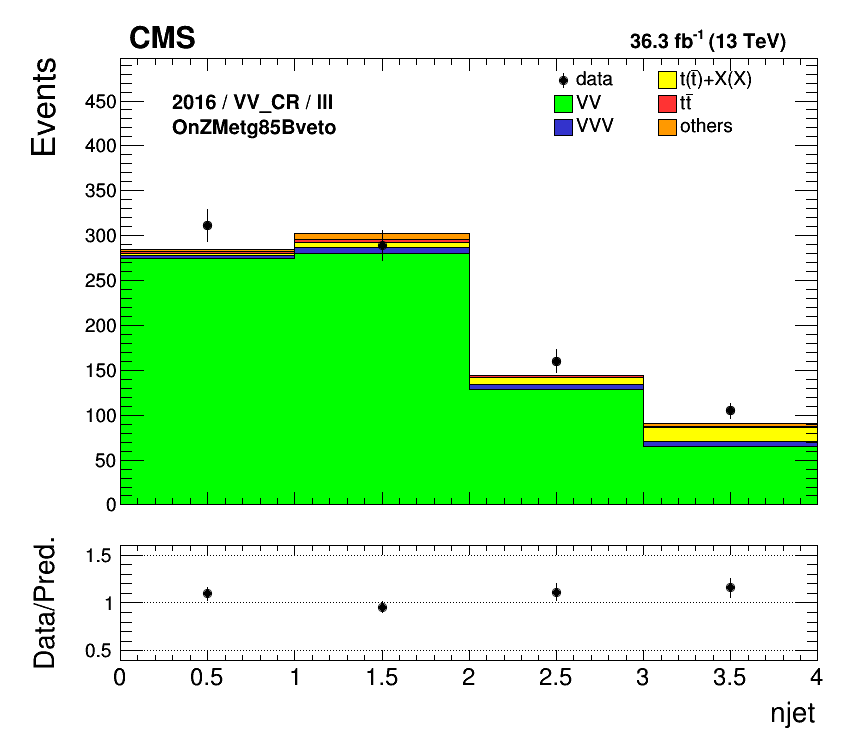
\includegraphics[width=0.325\textwidth]{figures/Part3/Systematics/njet_2016}&
    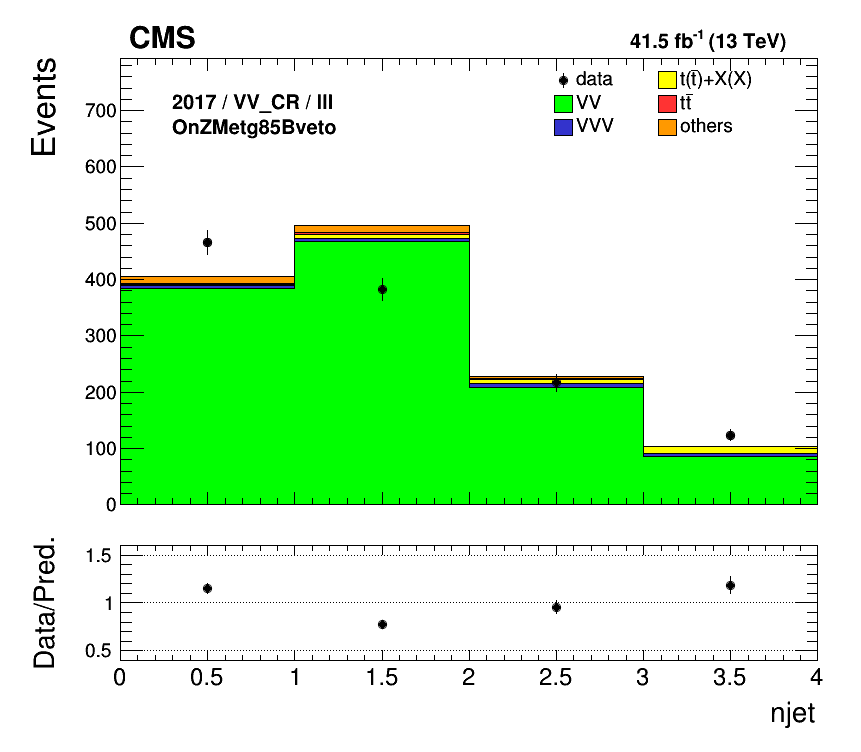
\includegraphics[width=0.325\textwidth]{figures/Part3/Systematics/njet_2017}&
  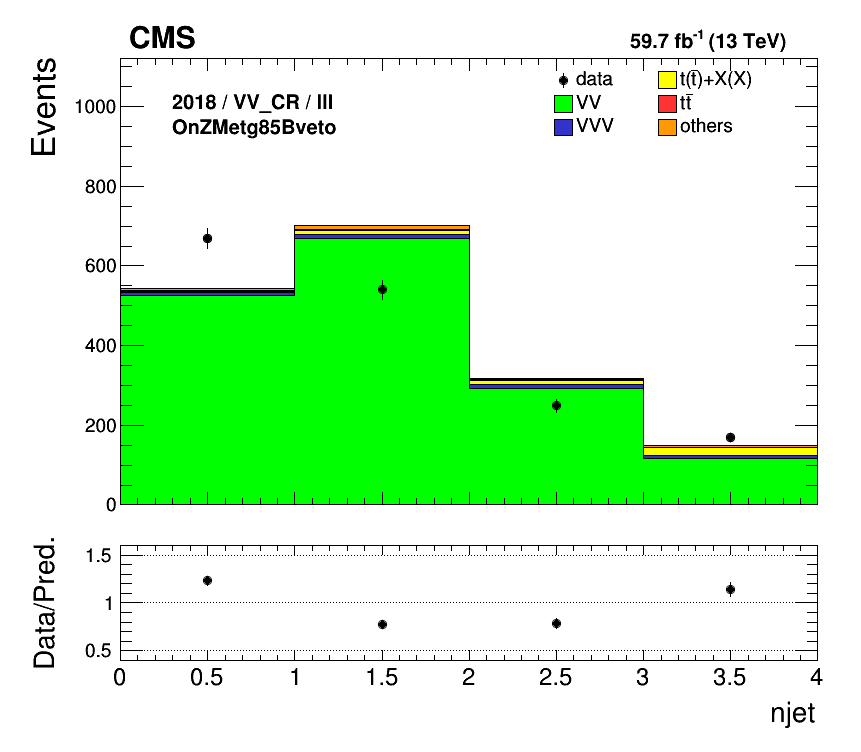
\includegraphics[width=0.325\textwidth]{figures/Part3/Systematics/njet_2018}\\
 \end{tabular}
 \caption{The diboson \acp{VR}, from left to right: 2016, 2017 and 2018 datasets.}
 \label{fig:VV_CR}
 \end{center}
\end{figure}

The scale factor $\epsilon$ is used to estimate the uncertainty, denoted by $\Delta$,

\begin{equation}
\Delta=|1-\epsilon|
\end{equation}

\begin{figure}[tbh!]
 \begin{center}
 \begin{tabular}{ccc}
  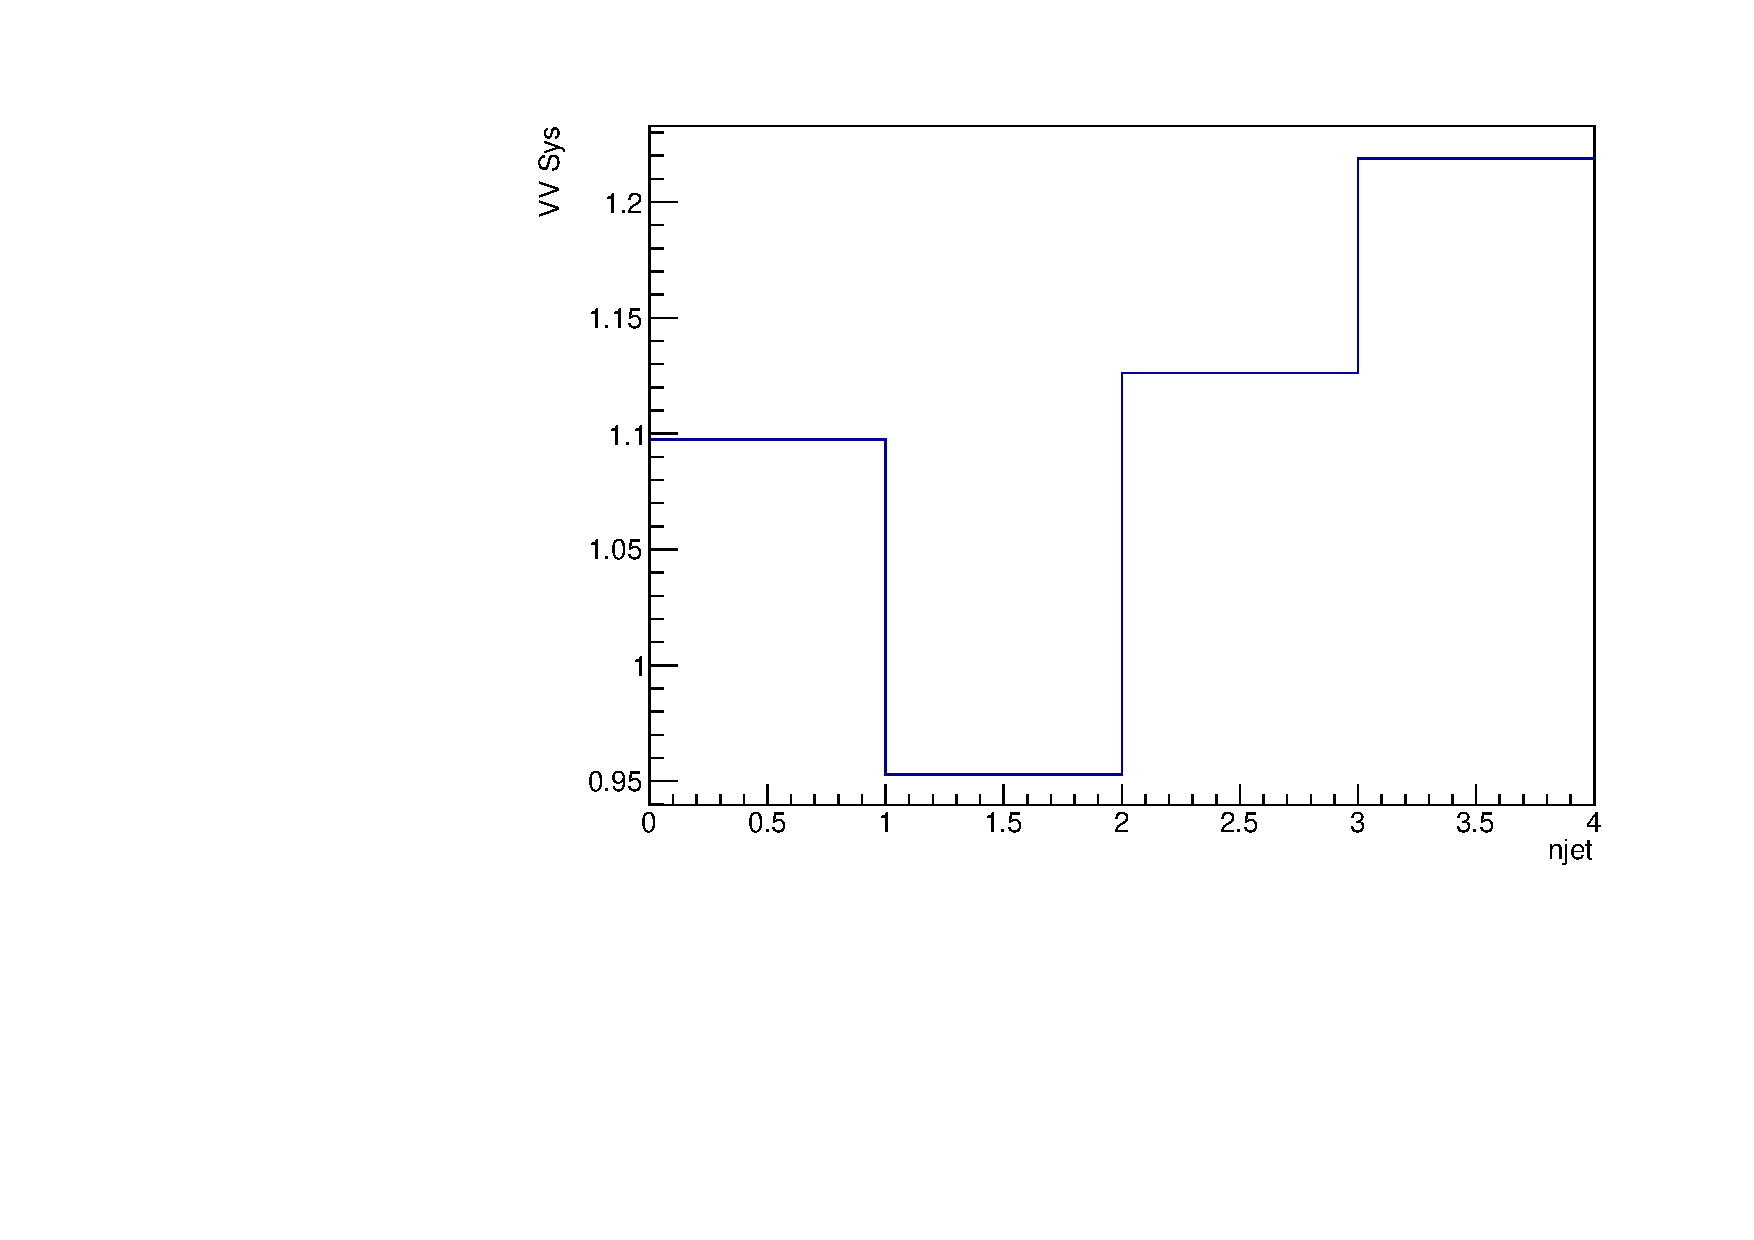
\includegraphics[width=0.325\textwidth]{figures/Part3/Systematics/2016_VV_Sys_1D}&
    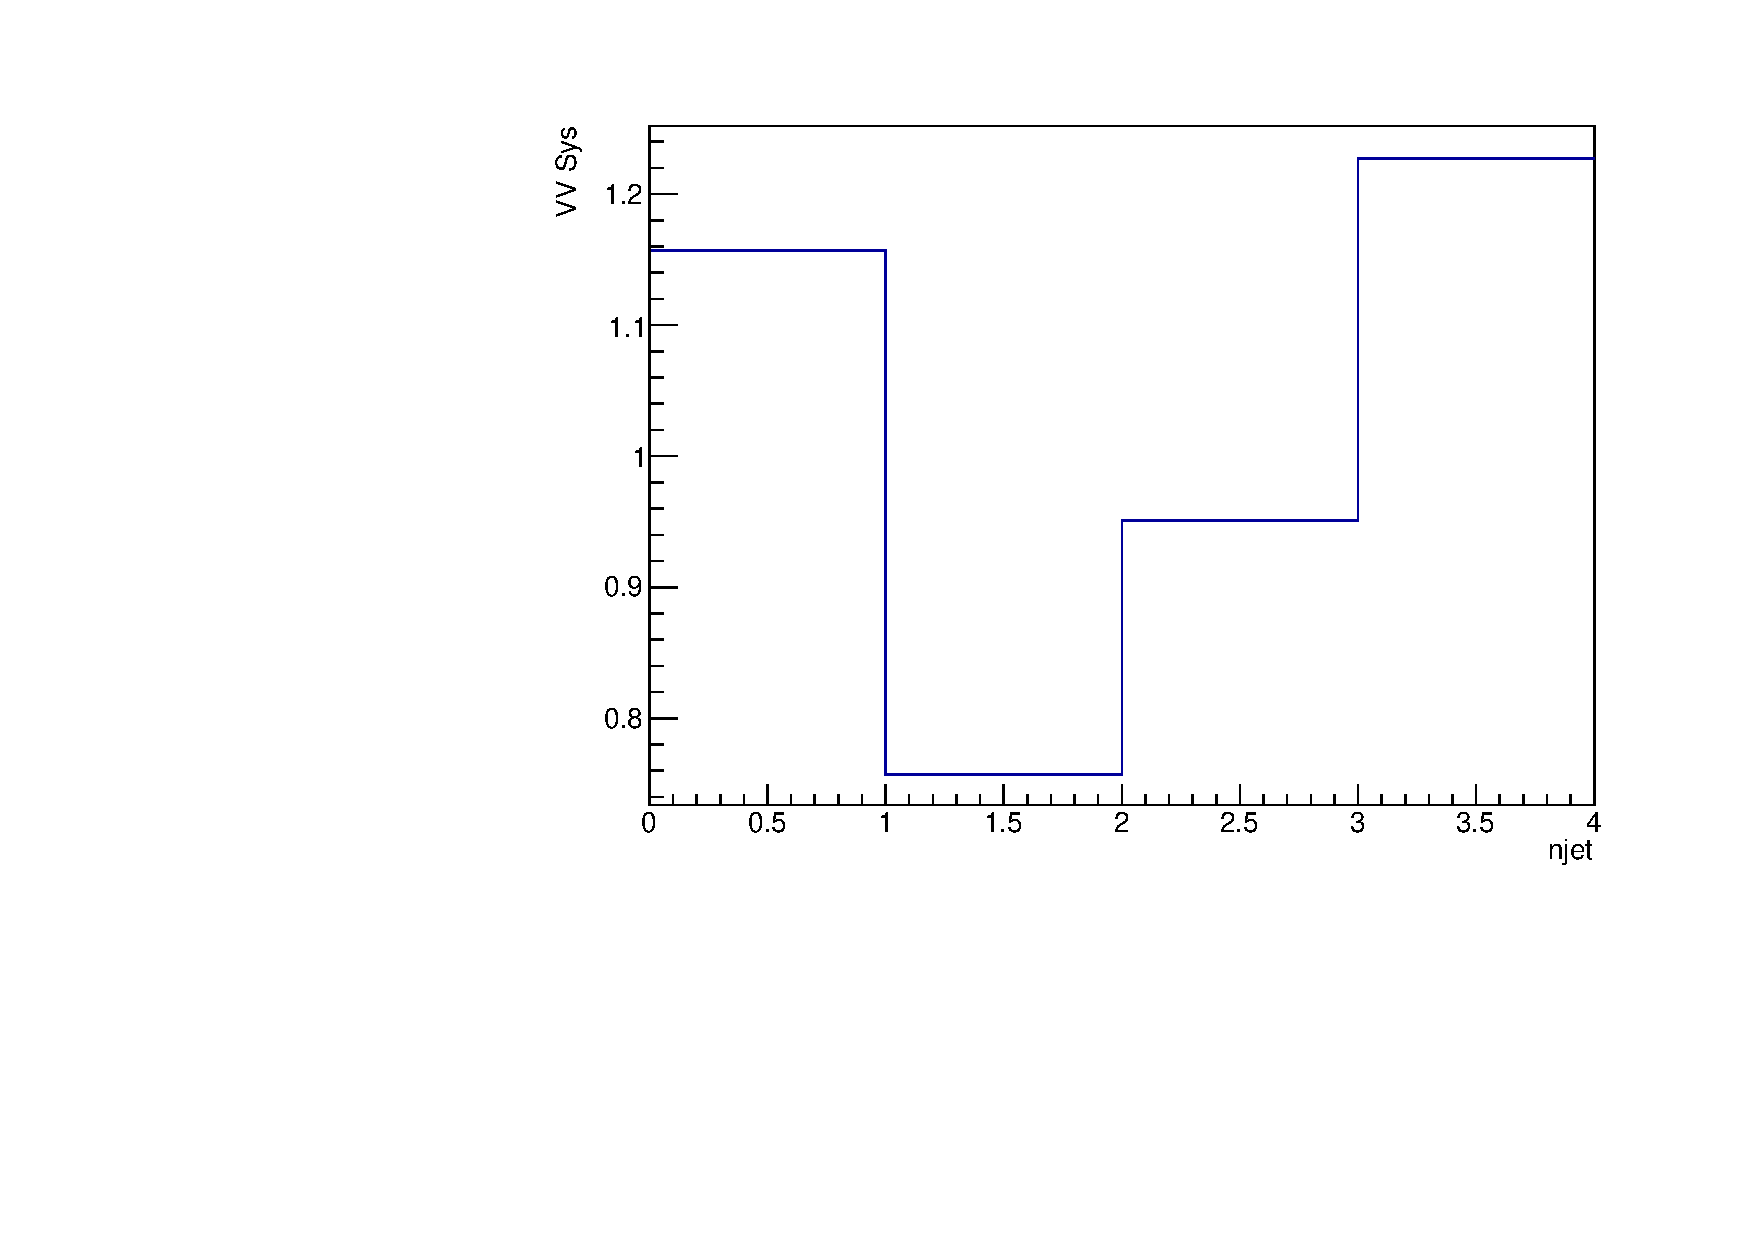
\includegraphics[width=0.325\textwidth]{figures/Part3/Systematics/2017_VV_Sys_1D}&
  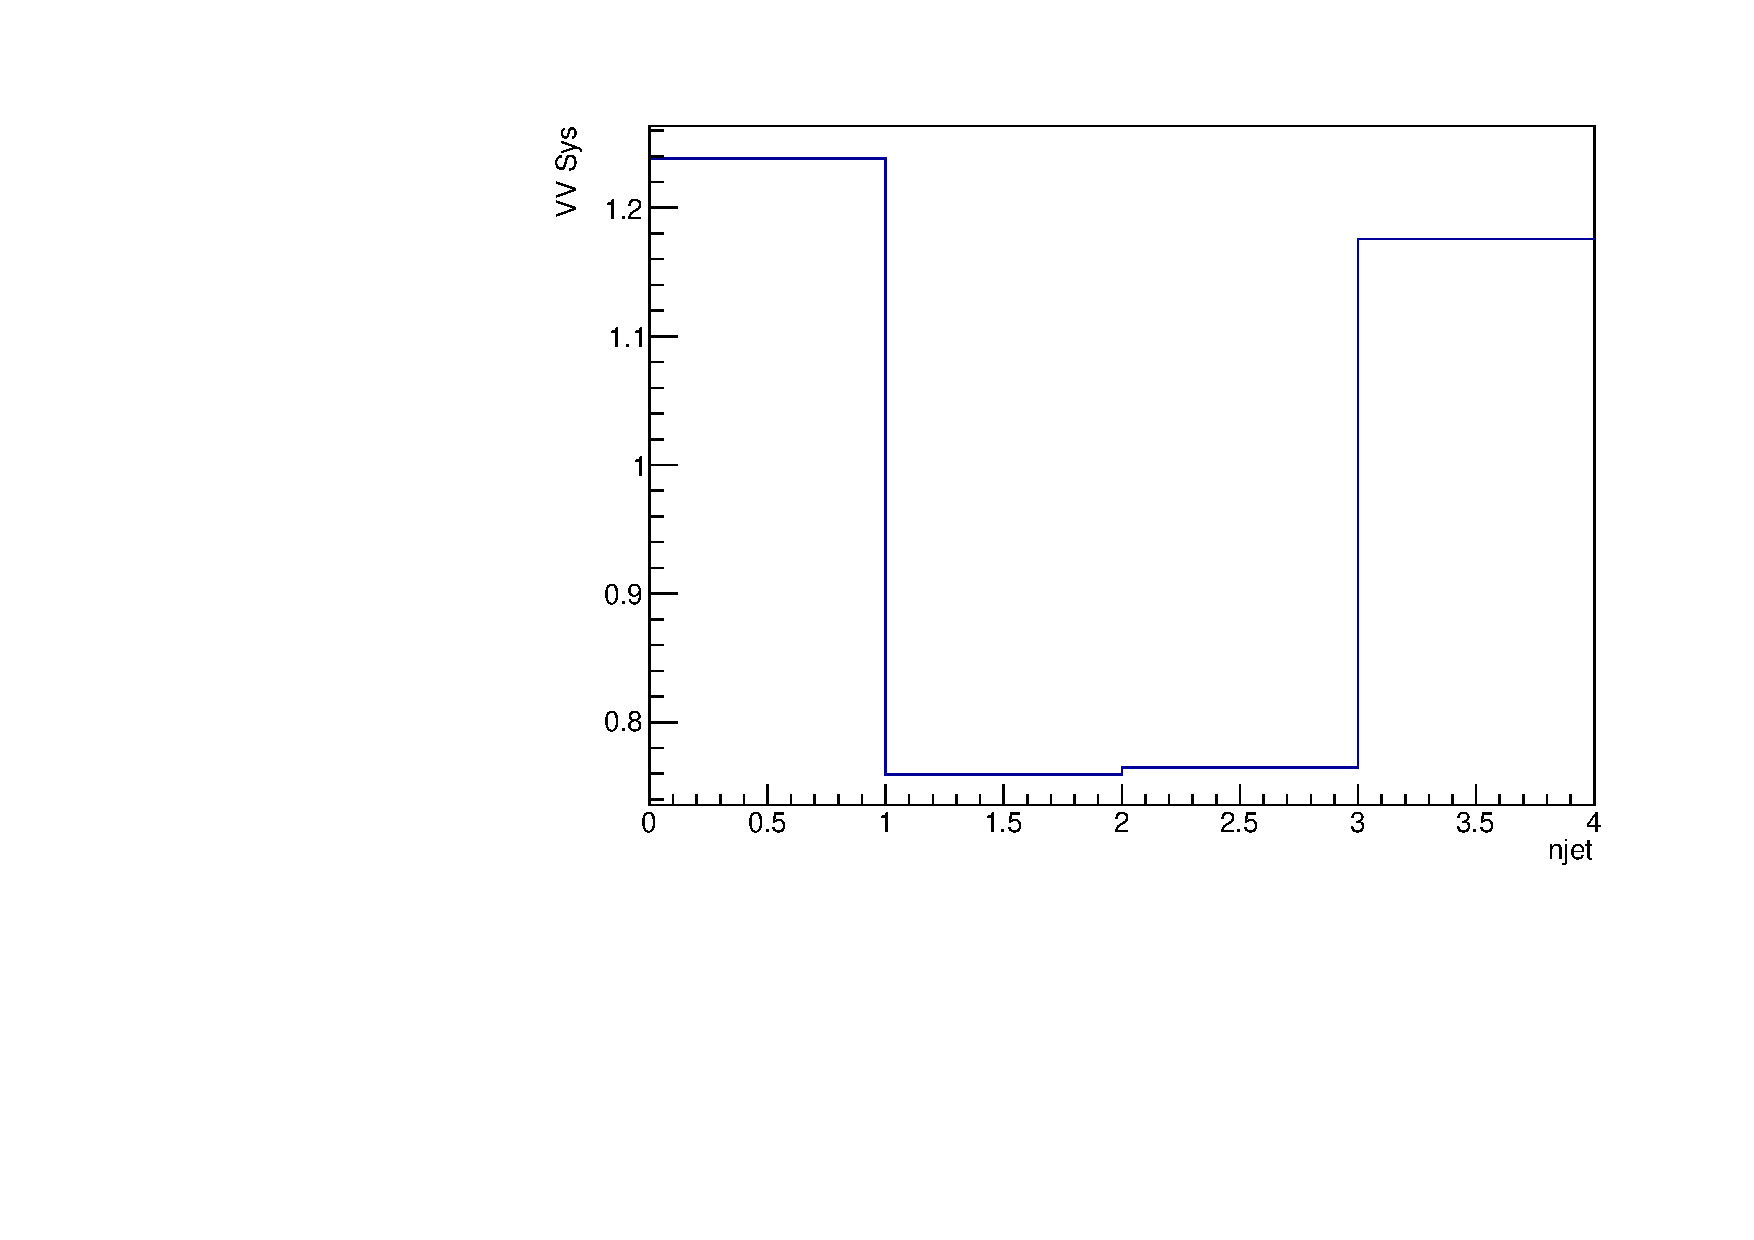
\includegraphics[width=0.325\textwidth]{figures/Part3/Systematics/2018_VV_Sys_1D}\\
 \end{tabular}
 \caption{Scale factors derived from the diboson \acp{VR}, from left to right: 2016, 2017 and 2018 datasets.}
 \label{fig:SF_VV}
 \end{center}
\end{figure}

This uncertainty shifts the predictions of WZ and ZZ processes by up to 20$\%$, as is shown in Figure \ref{fig:SF_VV}.
%%%%%%%%%%%%%%%%%%%%%%%%%%%%%%%%%%%%%%%%%%%%%%%%%%%%%%%%
%%%%%%%%%%%%%%%%%%%%%%%%%%%%%%%%%%%%%%%%%%%%%%%%%%%%%%%%

\section{Other Experimental Uncertainties}
\label{sec:OthUnc}

\begin{itemize}
\item Lepton reconstruction, identification, and isolation: electron/muon reconstruction uncertainties are provided by relevant POG. Uncertainties associated with lepton identification and isolation scale factors were evaluated by the authors of the mvaTOP ID cite{mvaTOP}. The statistical components of these uncertainties are treated as uncorrelated while the other components are treated as fully correlated. For high $p_{T}$ muons ($p_{T}>$200GeV), an additional uncertainty (denoted ``muIDHighPt") is assigned and it increases linearly from 0 to 10$\%$ (200GeV-1000GeV) and is caped at $10\%$ after 1000GeV.
\item Muon scale uncertainties: uncertainties on muon momentum (denoted ``MuonScale") are assigned using different method according to the muon $p_{T}$: Rochester algorithm is used for low $p_{T}$ muons ($p_{T}<$200Gev), while GEcite{GEmethod} method is used for high $p_T$ muons ($p_{T}>$200Gev).
\item b-tagging: b-tagging efficiency and uncertainty is provided by the BTV group. 
\item trigger scale factor: trigger scale factors are set to 1 and a flat 2$\%$ uncertainty is assigned. This uncertainty is treated as uncorrelated.
\item Luminosity: The uncertainties of 1.0$\%$, 2.0$\%$ and 1.5$\%$  are assigned to the integrated luminosity for 2016, 2017, 2018, respectively. When processing the run 2 data the individual year uncertainties are treated as uncorrelated while there are two additional correlated luminosity uncertainties; firstly, 0.6$\%$, 0.9$\%$ and 2.0$\%$ for each year respectively to account for the correlation between 2016, 2017 and 2018 data and secondly, 0.6$\%$,0.2$\%$ for 2017 and 2018 respectively to account for the correlation between 2017 and 2018 data. 
\item jet energy scale and resolution: The jet energy scale, JES, and jet energy resolution, JER, are centrally provided by the JET/MET POG cite{JEC}. Variations of jet energy scale and resolution are propagated to the MET and b-tagging SF.
\item pile-up reweighting: The measured minimum bias cross-section is varied up and down by 4.6$\%$. This uncertainty is treated as correlated. 
\item MET unclustered missing energy is considered and treated as uncorrelated across the years.
\item L1 ECAL prefiring: In the 2016 and 2017 datasets, L1 EGamma triggers fired early causing many uninteresting events to be recorded while the later interesting events were rejected. Since this effect is not present in the MC simulation, a tool cite{ECALPre} provided by the L1 DPG is used to reweight MC events. This uncertainty is treated as correlated. 
\item HEM15/16 Issue: The HEM15/16 issue refers to two HCAL modules whose power supply died in 
the middle of the data taking (runs$>=$319077, i.e. last certified run of 
2018B, and all of 2018C+D). The HEM issue is likely a very small effect but we still have to check it following the procedure in cite{HEM}
\end{itemize}

Uncertainties related to B-tagging scale factors are split into different sources. For b and udsg jets, we applied lf, hf, hfstats1/2, and lfstats1/2 uncertainties. For c jets, we applied cferr1/2 uncertainties. Correlations between different sources are specified in the Table~\ref{tab:btagsys}.

\begin{table}[!hbtp]
\sffamily
\centering
\caption{
A hyphen ($-$) denotes that a source is not correlated between the different years.
}
\begin{tabular}{lcl}
\toprule
Source & Correlated & Description\\
\midrule
lf			& \checkmark & udsg+c jets in heavy flavor region\\ %HF$^1$
hf			& \checkmark & b+c jets in light flavor region \\ %LF$^2$
hfstats1	& - 		 & Linear fluctuations of c jets\\
hfstats2	& -			 & Quadratic fluctuations of c jets \\
lfstats1	& -			 & Linear fluctuations of udsg jets \\
lfstats2	& -			 & Quadratic fluctuations of udsg jets \\
cferr1		& \checkmark & Linear fluctuations of c jets \\
cferr2		& \checkmark & Quadratic fluctuations of c jets \\
\bottomrule
\end{tabular}
\label{tab:btagsys}
\end{table}

\subsection{Jet energy scale uncertainties}

Uncertainties associated with JES are split into their 27 components and properly treated the correlations of the split uncertainties by year as recommended by the JETMET POG and described in the Table \ref{tab:jec}.

\begin{table}[!hbtp]
\sffamily
\centering
\caption{
Summary of the sources of uncertainty related to the JECs.
A hyphen ($-$) denotes that a source is not correlated between the different years.
}
\label{tab:jec}
\begin{tabular}{lc|lc}
\toprule
Source & Correlated & Source & Correlated \\
\midrule
AbsoluteStat			& -		&	 RelativePtHF			& \checkmark			 \\
AbsoluteScale			& \checkmark		&	 RelativeBal				& \checkmark			 \\
AbsoluteMPFBias			& \checkmark 	&	 RelativeSample			& -			 \\	 
Fragmentation			& \checkmark		&	 RelativeFSR				& -			 \\
SinglePionECAL			& \checkmark	&	 RelativeStatFSR			& \checkmark			 \\	 
SinglePionHCAL			& \checkmark	&	 RelativeStatEC			& -			 \\	 
FlavorQCD				& \checkmark	&	 RelativeStatHF			& -			 \\	 
TimePtEta				& -			 &          PileUpDataMC			& \checkmark			 \\
RelativeJEREC1			& -		&	    PileUpPtRef				& \checkmark			 \\
RelativeJEREC2			& -		&	    PileUpPtBB				& \checkmark			 \\
RelativeJERHF			& \checkmark		&	 PileUpPtEC1				& \checkmark			 \\
RelativePtBB			& \checkmark		&	 PileUpPtEC2				& \checkmark			 \\
RelativePtEC1			& -			&     PileUpPtHF				& \checkmark			 \\
RelativePtEC2			& -			&     & \\
\bottomrule
\end{tabular}
\end{table}

B-tagging scale factors and MET vector are computed for each of the JES templates and treated as uncertainties that are fully correlated to the respective JES sources. 

The overall systematic uncertainty on background is estimated to be about 15 $\%$ in SR.

 A comparison of different sources of systematic uncertainties of the background estimates in SR is shown in Figure \ref{fig:Comp_sys_background}.

\begin{figure}[tbh!]
 \begin{center}
 \begin{tabular}{cc}
    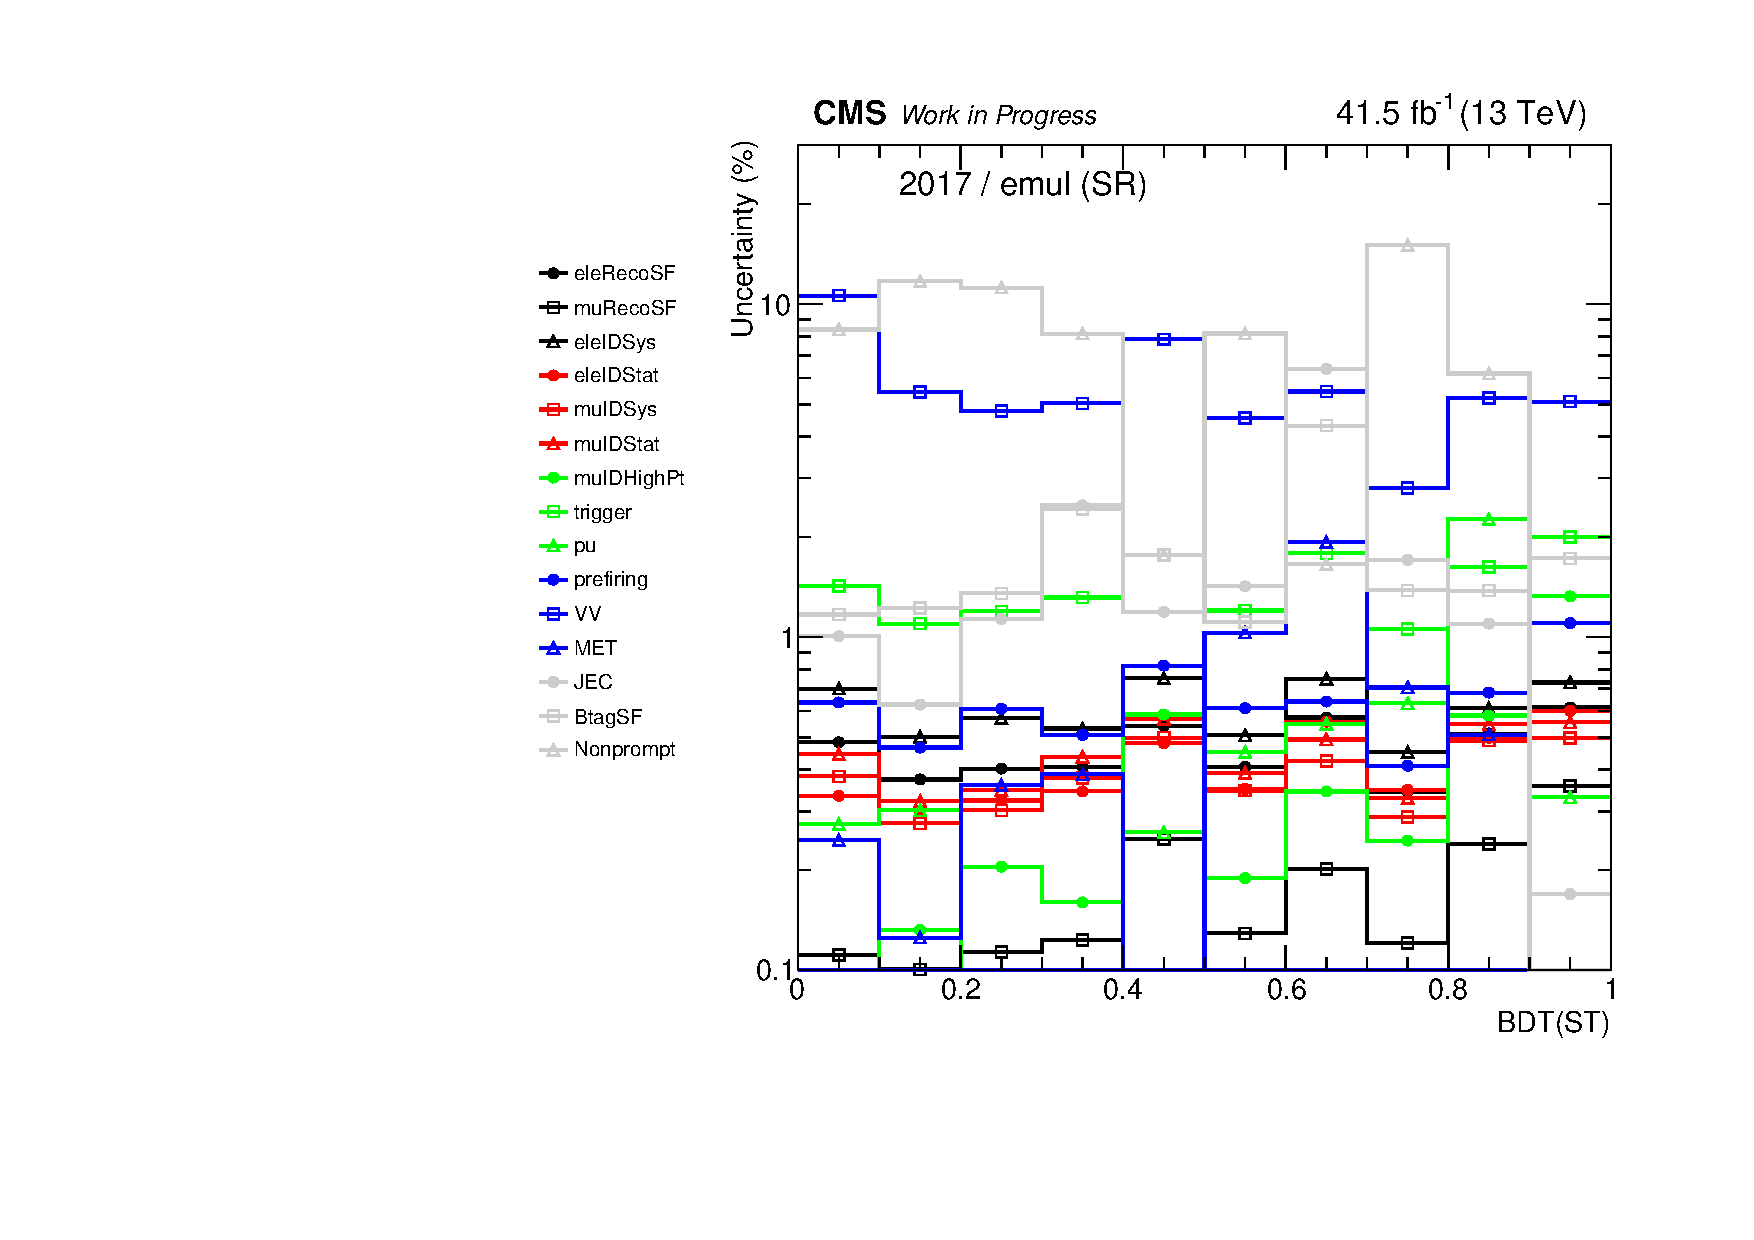
\includegraphics[width=0.45\textwidth]{figures/Part3/Systematics/sysBDT_ST_bkg_2017}&
  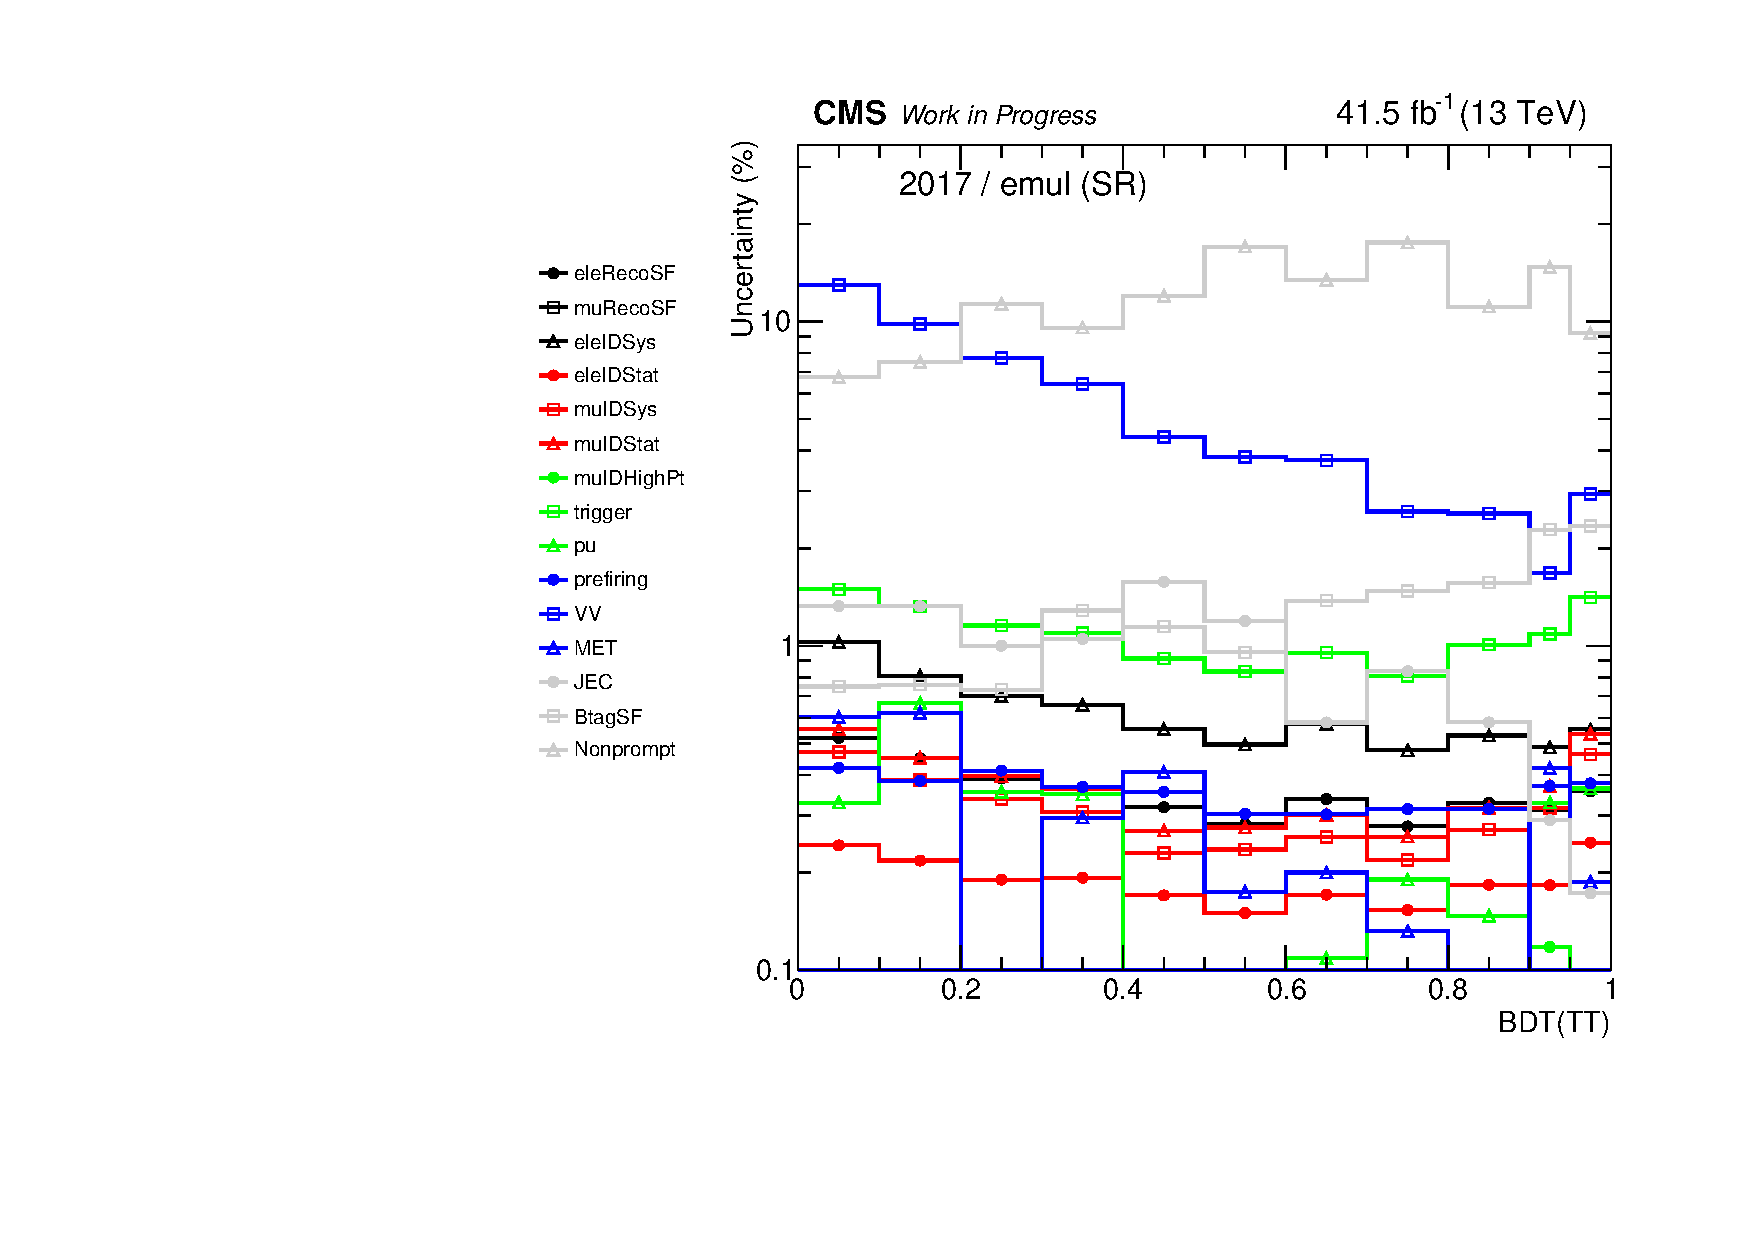
\includegraphics[width=0.45\textwidth]{figures/Part3/Systematics/sysBDT_TT_bkg_2017} \\
 \end{tabular}
 \caption{Distributions of relative uncertainties on total expected backgrounds as a function of BDT output in ST enriched SR (left), TT enriched SR (right). Luminosity and normalization uncertainties are not included in these plots. JES, JER and HEM are combined into "JEC". Sources of b-tagging uncertainties listed in Table~\ref{tab:btagsys} are combined into "BtagSF".}
 \label{fig:Comp_sys_background}
 \end{center}
\end{figure}

 A comparison of different sources of systematic uncertainties of the signal estimates in SR is shown in Figure \ref{fig:Comp_sys_signal}.

\begin{figure}[tbh!]
 \begin{center}
 \begin{tabular}{cc}
    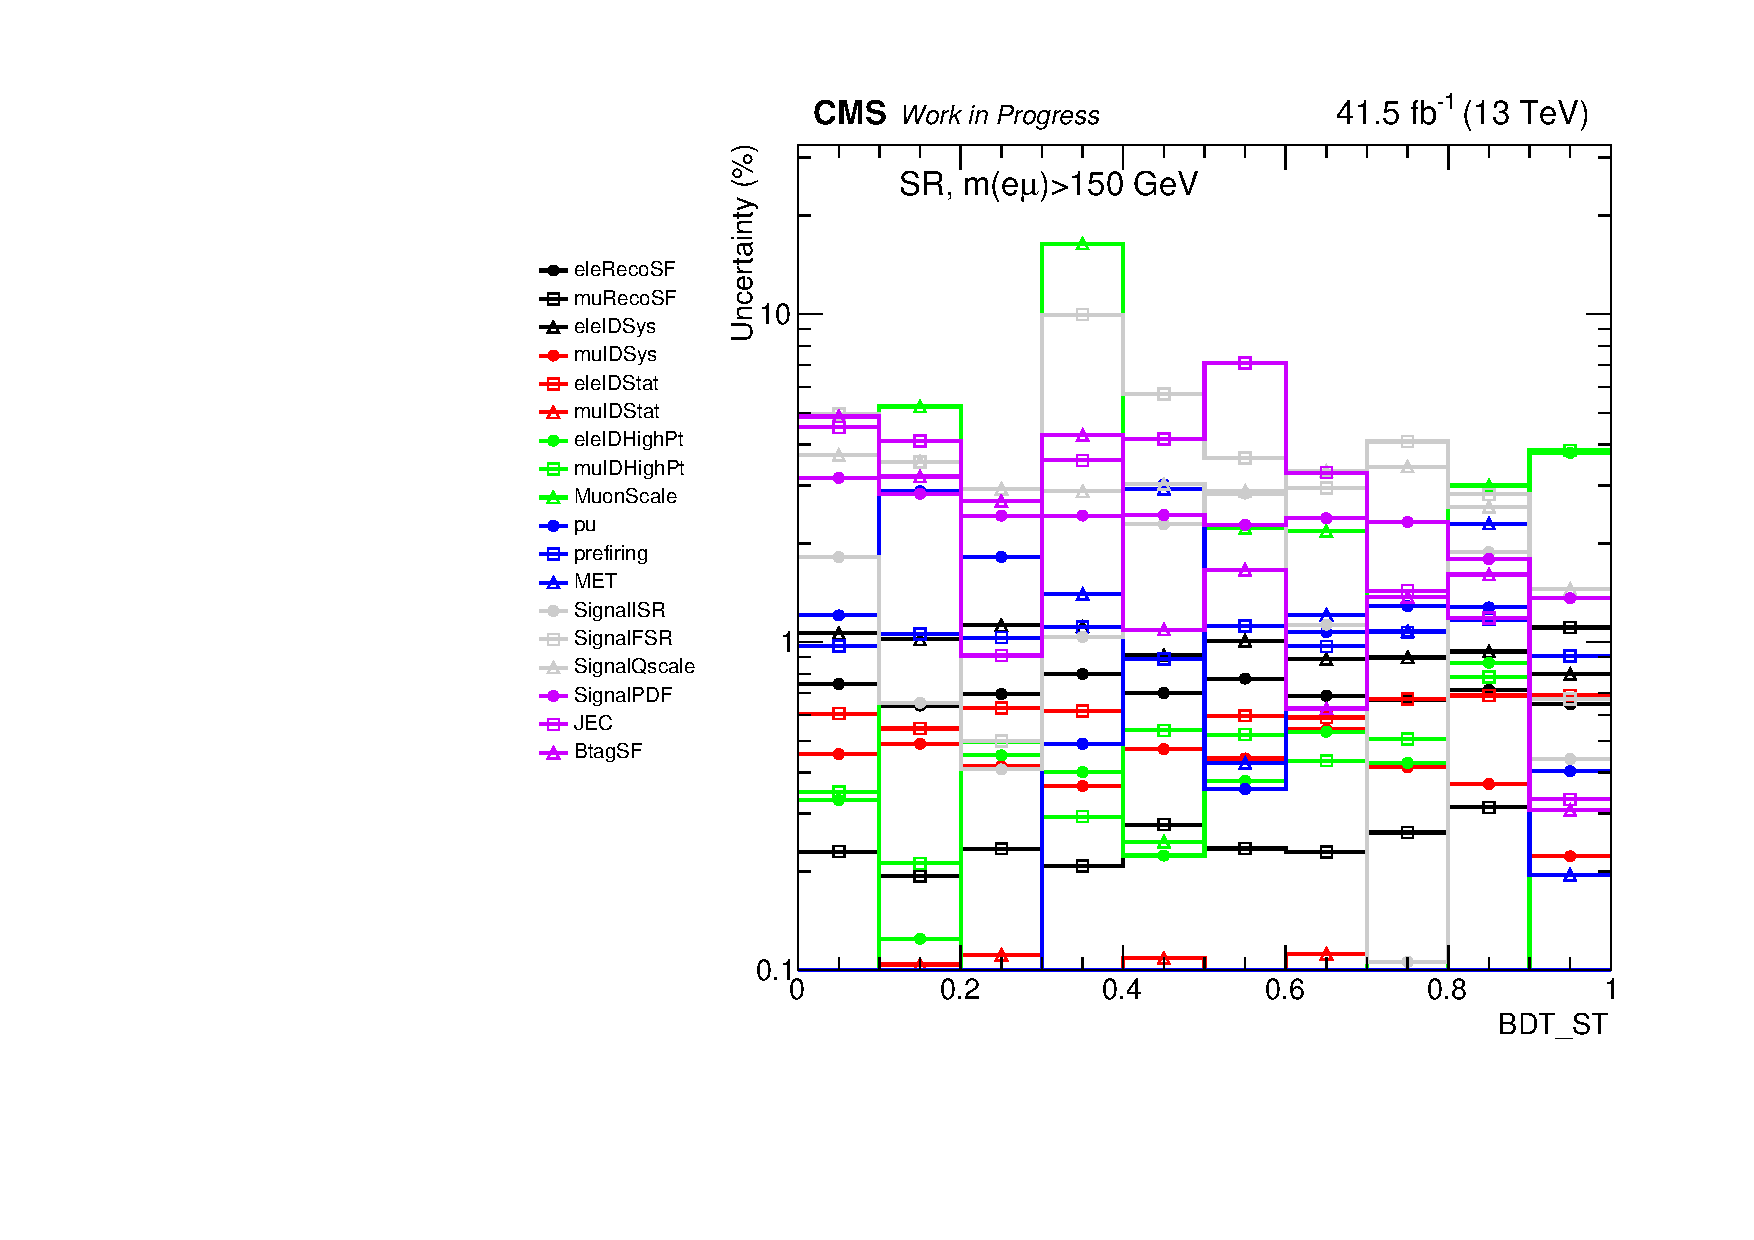
\includegraphics[width=0.45\textwidth]{figures/Part3/Systematics/sysBDT_ST_sig_2017}&
  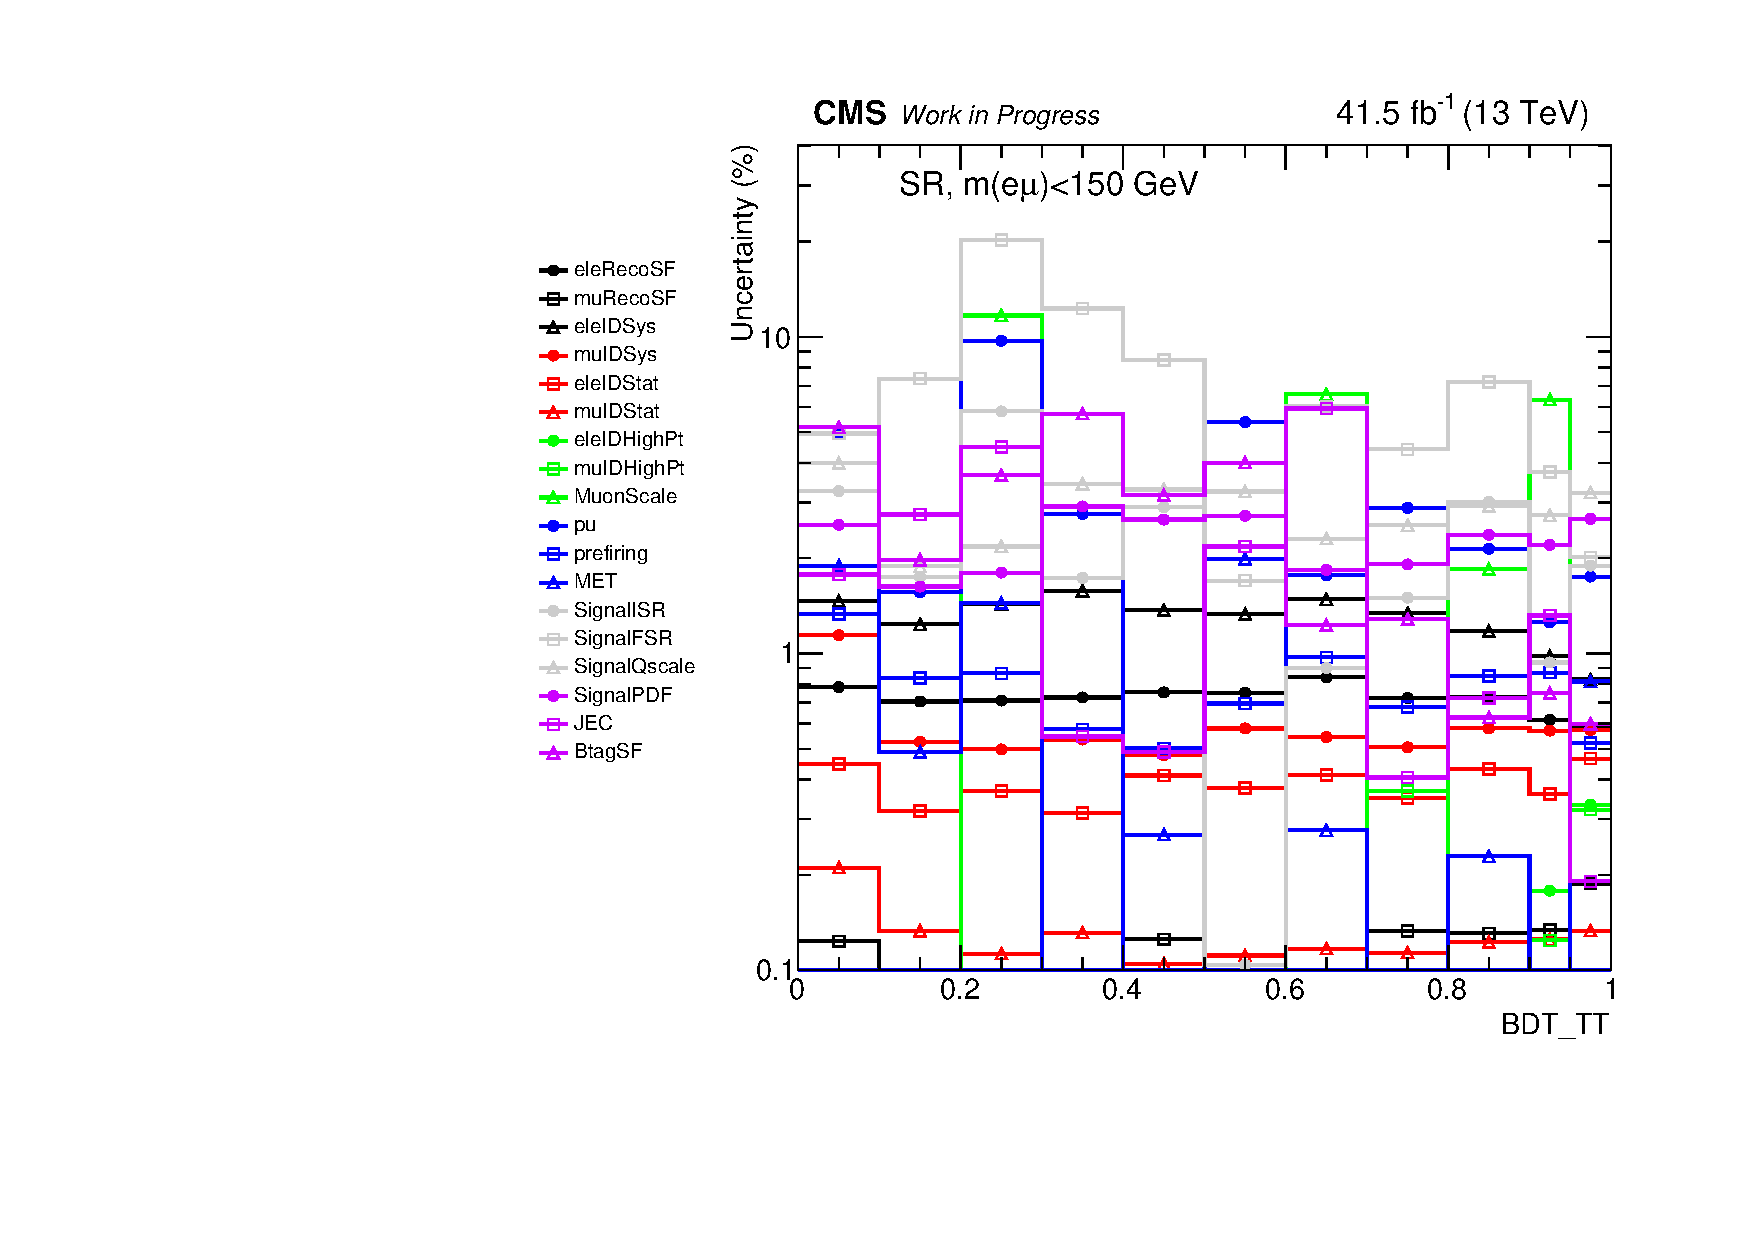
\includegraphics[width=0.45\textwidth]{figures/Part3/Systematics/sysBDT_TT_sig_2017} \\
 \end{tabular}
 \caption{Distributions of relative uncertainties on signal ($C_{e\mu tu}^{vector}$ is used as an example) as a function of BDT output in ST enriched SR (left), TT enriched SR (right). Luminosity and normalization uncertainties are not included in these plots. JES, JER and HEM are combined into "JEC". Sources of b-tagging uncertainties listed in Table~\ref{tab:btagsys} are combined into "BtagSF".}
 \label{fig:Comp_sys_signal}
 \end{center}
\end{figure}

Representative range of systematic uncertainties on background and signal MC samples are summarized in cite{SysError}. These uncertainties are extracted from the last bins of the BDT distribution.